\documentclass[twoside]{book}

% Packages required by doxygen
\usepackage{fixltx2e}
\usepackage{calc}
\usepackage{doxygen}
\usepackage[export]{adjustbox} % also loads graphicx
\usepackage{graphicx}
\usepackage[utf8]{inputenc}
\usepackage{makeidx}
\usepackage{multicol}
\usepackage{multirow}
\PassOptionsToPackage{warn}{textcomp}
\usepackage{textcomp}
\usepackage[nointegrals]{wasysym}
\usepackage[table]{xcolor}

% Font selection
\usepackage[T1]{fontenc}
\usepackage[scaled=.90]{helvet}
\usepackage{courier}
\usepackage{amssymb}
\usepackage{sectsty}
\renewcommand{\familydefault}{\sfdefault}
\allsectionsfont{%
  \fontseries{bc}\selectfont%
  \color{darkgray}%
}
\renewcommand{\DoxyLabelFont}{%
  \fontseries{bc}\selectfont%
  \color{darkgray}%
}
\newcommand{\+}{\discretionary{\mbox{\scriptsize$\hookleftarrow$}}{}{}}

% Page & text layout
\usepackage{geometry}
\geometry{%
  a4paper,%
  top=2.5cm,%
  bottom=2.5cm,%
  left=2.5cm,%
  right=2.5cm%
}
\tolerance=750
\hfuzz=15pt
\hbadness=750
\setlength{\emergencystretch}{15pt}
\setlength{\parindent}{0cm}
\setlength{\parskip}{3ex plus 2ex minus 2ex}
\makeatletter
\renewcommand{\paragraph}{%
  \@startsection{paragraph}{4}{0ex}{-1.0ex}{1.0ex}{%
    \normalfont\normalsize\bfseries\SS@parafont%
  }%
}
\renewcommand{\subparagraph}{%
  \@startsection{subparagraph}{5}{0ex}{-1.0ex}{1.0ex}{%
    \normalfont\normalsize\bfseries\SS@subparafont%
  }%
}
\makeatother

% Headers & footers
\usepackage{fancyhdr}
\pagestyle{fancyplain}
\fancyhead[LE]{\fancyplain{}{\bfseries\thepage}}
\fancyhead[CE]{\fancyplain{}{}}
\fancyhead[RE]{\fancyplain{}{\bfseries\leftmark}}
\fancyhead[LO]{\fancyplain{}{\bfseries\rightmark}}
\fancyhead[CO]{\fancyplain{}{}}
\fancyhead[RO]{\fancyplain{}{\bfseries\thepage}}
\fancyfoot[LE]{\fancyplain{}{}}
\fancyfoot[CE]{\fancyplain{}{}}
\fancyfoot[RE]{\fancyplain{}{\bfseries\scriptsize Generated by Doxygen }}
\fancyfoot[LO]{\fancyplain{}{\bfseries\scriptsize Generated by Doxygen }}
\fancyfoot[CO]{\fancyplain{}{}}
\fancyfoot[RO]{\fancyplain{}{}}
\renewcommand{\footrulewidth}{0.4pt}
\renewcommand{\chaptermark}[1]{%
  \markboth{#1}{}%
}
\renewcommand{\sectionmark}[1]{%
  \markright{\thesection\ #1}%
}

% Indices & bibliography
\usepackage{natbib}
\usepackage[titles]{tocloft}
\setcounter{tocdepth}{3}
\setcounter{secnumdepth}{5}
\makeindex

% Hyperlinks (required, but should be loaded last)
\usepackage{ifpdf}
\ifpdf
  \usepackage[pdftex,pagebackref=true]{hyperref}
\else
  \usepackage[ps2pdf,pagebackref=true]{hyperref}
\fi
\hypersetup{%
  colorlinks=true,%
  linkcolor=blue,%
  citecolor=blue,%
  unicode%
}

% Custom commands
\newcommand{\clearemptydoublepage}{%
  \newpage{\pagestyle{empty}\cleardoublepage}%
}

\usepackage{caption}
\captionsetup{labelsep=space,justification=centering,font={bf},singlelinecheck=off,skip=4pt,position=top}

%===== C O N T E N T S =====

\begin{document}

% Titlepage & ToC
\hypersetup{pageanchor=false,
             bookmarksnumbered=true,
             pdfencoding=unicode
            }
\pagenumbering{alph}
\begin{titlepage}
\vspace*{7cm}
\begin{center}%
{\Large My Project }\\
\vspace*{1cm}
{\large Generated by Doxygen 1.8.13}\\
\end{center}
\end{titlepage}
\clearemptydoublepage
\pagenumbering{roman}
\tableofcontents
\clearemptydoublepage
\pagenumbering{arabic}
\hypersetup{pageanchor=true}

%--- Begin generated contents ---
\chapter{Hierarchical Index}
\section{Class Hierarchy}
This inheritance list is sorted roughly, but not completely, alphabetically\+:\begin{DoxyCompactList}
\item \contentsline{section}{Check\+Connection}{\pageref{classCheckConnection}}{}
\item \contentsline{section}{compare}{\pageref{classcompare}}{}
\item \contentsline{section}{Device}{\pageref{classDevice}}{}
\item exception\begin{DoxyCompactList}
\item \contentsline{section}{My\+Exception}{\pageref{structMyException}}{}
\end{DoxyCompactList}
\item \contentsline{section}{Feedback}{\pageref{classFeedback}}{}
\item \contentsline{section}{Get\+History}{\pageref{classGetHistory}}{}
\item \contentsline{section}{Get\+Local\+Devices}{\pageref{classGetLocalDevices}}{}
\item \contentsline{section}{Get\+OS}{\pageref{classGetOS}}{}
\item \contentsline{section}{Get\+Remote\+Config}{\pageref{classGetRemoteConfig}}{}
\item \contentsline{section}{H\+T\+T\+P\+Downloader}{\pageref{classHTTPDownloader}}{}
\item \contentsline{section}{Linux\+Conf}{\pageref{classLinuxConf}}{}
\item Q\+Dialog\begin{DoxyCompactList}
\item \contentsline{section}{Notebook\+G\+UI}{\pageref{classNotebookGUI}}{}
\end{DoxyCompactList}
\item Q\+Message\+Box\begin{DoxyCompactList}
\item \contentsline{section}{Question\+Box}{\pageref{classQuestionBox}}{}
\end{DoxyCompactList}
\item \contentsline{section}{qt\+\_\+meta\+\_\+stringdata\+\_\+\+Console\+Tab\+\_\+t}{\pageref{structqt__meta__stringdata__ConsoleTab__t}}{}
\item \contentsline{section}{qt\+\_\+meta\+\_\+stringdata\+\_\+\+Contributor\+Tab2\+\_\+t}{\pageref{structqt__meta__stringdata__ContributorTab2__t}}{}
\item \contentsline{section}{qt\+\_\+meta\+\_\+stringdata\+\_\+intro\+Tab\+\_\+t}{\pageref{structqt__meta__stringdata__introTab__t}}{}
\item \contentsline{section}{qt\+\_\+meta\+\_\+stringdata\+\_\+\+Notebook\+G\+U\+I\+\_\+t}{\pageref{structqt__meta__stringdata__NotebookGUI__t}}{}
\item \contentsline{section}{qt\+\_\+meta\+\_\+stringdata\+\_\+\+Restore\+Tab\+\_\+t}{\pageref{structqt__meta__stringdata__RestoreTab__t}}{}
\item \contentsline{section}{qt\+\_\+meta\+\_\+stringdata\+\_\+\+Run\+Tab\+\_\+t}{\pageref{structqt__meta__stringdata__RunTab__t}}{}
\item Q\+Widget\begin{DoxyCompactList}
\item \contentsline{section}{Console\+Tab}{\pageref{classConsoleTab}}{}
\item \contentsline{section}{Contributor\+Tab2}{\pageref{classContributorTab2}}{}
\item \contentsline{section}{intro\+Tab}{\pageref{classintroTab}}{}
\item \contentsline{section}{Restore\+Tab}{\pageref{classRestoreTab}}{}
\item \contentsline{section}{Run\+Tab}{\pageref{classRunTab}}{}
\end{DoxyCompactList}
\item \contentsline{section}{Restore\+G\+UI}{\pageref{classRestoreGUI}}{}
\item \contentsline{section}{Run\+Config}{\pageref{classRunConfig}}{}
\end{DoxyCompactList}

\chapter{Class Index}
\section{Class List}
Here are the classes, structs, unions and interfaces with brief descriptions\+:\begin{DoxyCompactList}
\item\contentsline{section}{\hyperlink{classCheckConnection}{Check\+Connection} }{\pageref{classCheckConnection}}{}
\item\contentsline{section}{\hyperlink{classcompare}{compare} }{\pageref{classcompare}}{}
\item\contentsline{section}{\hyperlink{classConsoleTab}{Console\+Tab} }{\pageref{classConsoleTab}}{}
\item\contentsline{section}{\hyperlink{classContributorTab2}{Contributor\+Tab2} }{\pageref{classContributorTab2}}{}
\item\contentsline{section}{\hyperlink{classDevice}{Device} }{\pageref{classDevice}}{}
\item\contentsline{section}{\hyperlink{classFeedback}{Feedback} }{\pageref{classFeedback}}{}
\item\contentsline{section}{\hyperlink{classGetHistory}{Get\+History} }{\pageref{classGetHistory}}{}
\item\contentsline{section}{\hyperlink{classGetLocalDevices}{Get\+Local\+Devices} }{\pageref{classGetLocalDevices}}{}
\item\contentsline{section}{\hyperlink{classGetOS}{Get\+OS} }{\pageref{classGetOS}}{}
\item\contentsline{section}{\hyperlink{classGetRemoteConfig}{Get\+Remote\+Config} }{\pageref{classGetRemoteConfig}}{}
\item\contentsline{section}{\hyperlink{classHTTPDownloader}{H\+T\+T\+P\+Downloader} }{\pageref{classHTTPDownloader}}{}
\item\contentsline{section}{\hyperlink{classintroTab}{intro\+Tab} }{\pageref{classintroTab}}{}
\item\contentsline{section}{\hyperlink{classLinuxConf}{Linux\+Conf} }{\pageref{classLinuxConf}}{}
\item\contentsline{section}{\hyperlink{structMyException}{My\+Exception} \\*Exception handling class }{\pageref{structMyException}}{}
\item\contentsline{section}{\hyperlink{classNotebookGUI}{Notebook\+G\+UI} }{\pageref{classNotebookGUI}}{}
\item\contentsline{section}{\hyperlink{structqt__meta__stringdata__ConsoleTab__t}{qt\+\_\+meta\+\_\+stringdata\+\_\+\+Console\+Tab\+\_\+t} }{\pageref{structqt__meta__stringdata__ConsoleTab__t}}{}
\item\contentsline{section}{\hyperlink{structqt__meta__stringdata__ContributorTab2__t}{qt\+\_\+meta\+\_\+stringdata\+\_\+\+Contributor\+Tab2\+\_\+t} }{\pageref{structqt__meta__stringdata__ContributorTab2__t}}{}
\item\contentsline{section}{\hyperlink{structqt__meta__stringdata__introTab__t}{qt\+\_\+meta\+\_\+stringdata\+\_\+intro\+Tab\+\_\+t} }{\pageref{structqt__meta__stringdata__introTab__t}}{}
\item\contentsline{section}{\hyperlink{structqt__meta__stringdata__NotebookGUI__t}{qt\+\_\+meta\+\_\+stringdata\+\_\+\+Notebook\+G\+U\+I\+\_\+t} }{\pageref{structqt__meta__stringdata__NotebookGUI__t}}{}
\item\contentsline{section}{\hyperlink{structqt__meta__stringdata__RestoreTab__t}{qt\+\_\+meta\+\_\+stringdata\+\_\+\+Restore\+Tab\+\_\+t} }{\pageref{structqt__meta__stringdata__RestoreTab__t}}{}
\item\contentsline{section}{\hyperlink{structqt__meta__stringdata__RunTab__t}{qt\+\_\+meta\+\_\+stringdata\+\_\+\+Run\+Tab\+\_\+t} }{\pageref{structqt__meta__stringdata__RunTab__t}}{}
\item\contentsline{section}{\hyperlink{classQuestionBox}{Question\+Box} }{\pageref{classQuestionBox}}{}
\item\contentsline{section}{\hyperlink{classRestoreGUI}{Restore\+G\+UI} }{\pageref{classRestoreGUI}}{}
\item\contentsline{section}{\hyperlink{classRestoreTab}{Restore\+Tab} }{\pageref{classRestoreTab}}{}
\item\contentsline{section}{\hyperlink{classRunConfig}{Run\+Config} }{\pageref{classRunConfig}}{}
\item\contentsline{section}{\hyperlink{classRunTab}{Run\+Tab} }{\pageref{classRunTab}}{}
\end{DoxyCompactList}

\chapter{Class Documentation}
\hypertarget{classCheckConnection}{}\section{Check\+Connection Class Reference}
\label{classCheckConnection}\index{Check\+Connection@{Check\+Connection}}
\subsection*{Static Public Member Functions}
\begin{DoxyCompactItemize}
\item 
\mbox{\Hypertarget{classCheckConnection_a1c4c6ce94485bd09f815b238a696527e}\label{classCheckConnection_a1c4c6ce94485bd09f815b238a696527e}} 
static bool \hyperlink{classCheckConnection_a1c4c6ce94485bd09f815b238a696527e}{Check\+Network} ()
\begin{DoxyCompactList}\small\item\em checks a network connection by downloading from google. \end{DoxyCompactList}\end{DoxyCompactItemize}


The documentation for this class was generated from the following files\+:\begin{DoxyCompactItemize}
\item 
Check\+Connection.\+h\item 
Check\+Connection.\+cpp\end{DoxyCompactItemize}

\hypertarget{classcompare}{}\section{compare Class Reference}
\label{classcompare}\index{compare@{compare}}
\subsection*{Public Member Functions}
\begin{DoxyCompactItemize}
\item 
\mbox{\Hypertarget{classcompare_ab6a31eca674772d2ce4a08d67c7c66eb}\label{classcompare_ab6a31eca674772d2ce4a08d67c7c66eb}} 
bool {\bfseries operator()} (\hyperlink{classDevice}{Device} lhs, \hyperlink{classDevice}{Device} rhs)
\item 
\mbox{\Hypertarget{classcompare_a770655d961911a14eb479c74a7a94992}\label{classcompare_a770655d961911a14eb479c74a7a94992}} 
bool {\bfseries operator()} (const \hyperlink{classDevice}{Device} lhs, const \hyperlink{classDevice}{Device} rhs) const
\item 
\mbox{\Hypertarget{classcompare_a7389f58eb67313e0984d63218941833d}\label{classcompare_a7389f58eb67313e0984d63218941833d}} 
bool {\bfseries operator$<$} (\hyperlink{classDevice}{Device} \&lhs)
\item 
\mbox{\Hypertarget{classcompare_a177684fa3fd487882edc1878965f23bc}\label{classcompare_a177684fa3fd487882edc1878965f23bc}} 
bool {\bfseries operator$<$} (const \hyperlink{classDevice}{Device} \&lhs) const
\end{DoxyCompactItemize}


The documentation for this class was generated from the following file\+:\begin{DoxyCompactItemize}
\item 
compare.\+h\end{DoxyCompactItemize}

\hypertarget{classConsoleTab}{}\section{Console\+Tab Class Reference}
\label{classConsoleTab}\index{Console\+Tab@{Console\+Tab}}


Inheritance diagram for Console\+Tab\+:\nopagebreak
\begin{figure}[H]
\begin{center}
\leavevmode
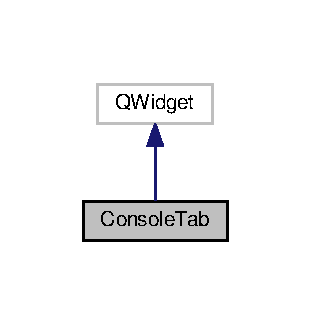
\includegraphics[width=149pt]{classConsoleTab__inherit__graph}
\end{center}
\end{figure}


Collaboration diagram for Console\+Tab\+:\nopagebreak
\begin{figure}[H]
\begin{center}
\leavevmode
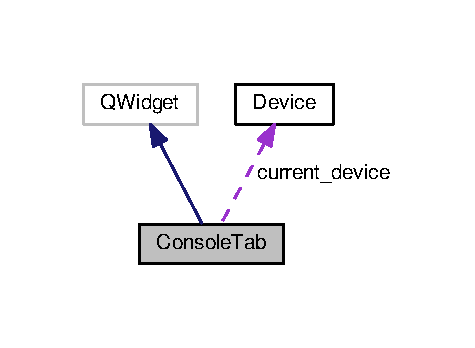
\includegraphics[width=228pt]{classConsoleTab__coll__graph}
\end{center}
\end{figure}
\subsection*{Public Slots}
\begin{DoxyCompactItemize}
\item 
void \hyperlink{classConsoleTab_abda9ef659782544e72f0e4561c5583f0}{show\+Buttons} (vector$<$ string $>$ details, bool success)
\item 
void \hyperlink{classConsoleTab_a695bb64854ca658dc9cc0a44c7a08f2c}{send\+To\+Console} (\hyperlink{classDevice}{Device} device, string method, vector$<$ string $>$ parameters)
\begin{DoxyCompactList}\small\item\em \hyperlink{classConsoleTab_a695bb64854ca658dc9cc0a44c7a08f2c}{Console\+Tab\+::send\+To\+Console}. \end{DoxyCompactList}\end{DoxyCompactItemize}
\subsection*{Signals}
\begin{DoxyCompactItemize}
\item 
\mbox{\Hypertarget{classConsoleTab_afbcbf3f97fa59e43aa9fe86c9549ebed}\label{classConsoleTab_afbcbf3f97fa59e43aa9fe86c9549ebed}} 
void {\bfseries set\+Tab} (int)
\item 
\mbox{\Hypertarget{classConsoleTab_a741773c43f4a548ffd154022429a3830}\label{classConsoleTab_a741773c43f4a548ffd154022429a3830}} 
void {\bfseries update\+Screen} ()
\item 
\mbox{\Hypertarget{classConsoleTab_a34925515a836a363cf85b25860c795d6}\label{classConsoleTab_a34925515a836a363cf85b25860c795d6}} 
void {\bfseries refresh\+Restore} (string)
\item 
\mbox{\Hypertarget{classConsoleTab_af58a230f2f192469205839920dd7fa66}\label{classConsoleTab_af58a230f2f192469205839920dd7fa66}} 
void {\bfseries send\+Reboot} ()
\end{DoxyCompactItemize}
\subsection*{Public Member Functions}
\begin{DoxyCompactItemize}
\item 
\hyperlink{classConsoleTab_a2c631d14f9fe5957e0622e10269e5115}{Console\+Tab} (Q\+Widget $\ast$m\+\_\+parent)
\item 
\mbox{\Hypertarget{classConsoleTab_aa2b97a380a10d6100dc956d150ebd590}\label{classConsoleTab_aa2b97a380a10d6100dc956d150ebd590}} 
void {\bfseries set\+Device} (\hyperlink{classDevice}{Device} device)
\item 
void \hyperlink{classConsoleTab_a7b2d0987db00c8b9af7ece7b36a82624}{fails\+\_\+result} ()
\item 
void \hyperlink{classConsoleTab_a866367073a3150527988f7cb841d5002}{works\+\_\+result} ()
\item 
\mbox{\Hypertarget{classConsoleTab_a312dd40624d78a7d8506f97eb837c492}\label{classConsoleTab_a312dd40624d78a7d8506f97eb837c492}} 
void \hyperlink{classConsoleTab_a312dd40624d78a7d8506f97eb837c492}{Reboot\+Machine} ()
\begin{DoxyCompactList}\small\item\em Reboots the machine. \end{DoxyCompactList}\item 
void \hyperlink{classConsoleTab_aae70e23b23e401b219edefcac4882eaf}{clear\+Layout} (Q\+Layout $\ast$layout, bool delete\+Widgets)
\begin{DoxyCompactList}\small\item\em \hyperlink{classConsoleTab_aae70e23b23e401b219edefcac4882eaf}{Console\+Tab\+::clear\+Layout}. \end{DoxyCompactList}\end{DoxyCompactItemize}
\subsection*{Public Attributes}
\begin{DoxyCompactItemize}
\item 
\mbox{\Hypertarget{classConsoleTab_ad37d80565e56f70da9774947e5cbe4cf}\label{classConsoleTab_ad37d80565e56f70da9774947e5cbe4cf}} 
Q\+Widget $\ast$ {\bfseries parent}
\item 
\mbox{\Hypertarget{classConsoleTab_a0304aee81920bf219e17ba6531a4119e}\label{classConsoleTab_a0304aee81920bf219e17ba6531a4119e}} 
Q\+Term\+Widget $\ast$ {\bfseries console}
\item 
\mbox{\Hypertarget{classConsoleTab_aa4213b0dd52a74260783e0a46feadee6}\label{classConsoleTab_aa4213b0dd52a74260783e0a46feadee6}} 
Q\+Grid\+Layout $\ast$ {\bfseries main\+Layout}
\item 
\mbox{\Hypertarget{classConsoleTab_aa771347a9e50ee2880a2f45afc9807f3}\label{classConsoleTab_aa771347a9e50ee2880a2f45afc9807f3}} 
Q\+Push\+Button $\ast$ {\bfseries works\+\_\+button}
\item 
\mbox{\Hypertarget{classConsoleTab_abf0343f21a612a41948b275e348bf29f}\label{classConsoleTab_abf0343f21a612a41948b275e348bf29f}} 
Q\+Push\+Button $\ast$ {\bfseries fails\+\_\+button}
\item 
\mbox{\Hypertarget{classConsoleTab_a4d68ba1e38f3633ed8bcb3ada17219dc}\label{classConsoleTab_a4d68ba1e38f3633ed8bcb3ada17219dc}} 
Q\+Label $\ast$ {\bfseries success\+\_\+label}
\item 
\mbox{\Hypertarget{classConsoleTab_a67b2d7ba4daabcd8bac8187a035c79fc}\label{classConsoleTab_a67b2d7ba4daabcd8bac8187a035c79fc}} 
Q\+Label $\ast$ {\bfseries reboot\+\_\+label}
\item 
\mbox{\Hypertarget{classConsoleTab_ad4de3b850b9638c177925970ec3495d3}\label{classConsoleTab_ad4de3b850b9638c177925970ec3495d3}} 
Q\+Label $\ast$ {\bfseries done\+\_\+label}
\item 
\mbox{\Hypertarget{classConsoleTab_abac4c2031895f3bd40e2a81dcb67be7c}\label{classConsoleTab_abac4c2031895f3bd40e2a81dcb67be7c}} 
Q\+Push\+Button $\ast$ {\bfseries reboot\+\_\+button}
\item 
\mbox{\Hypertarget{classConsoleTab_a26ca4389db3dec2aa5992491580c86be}\label{classConsoleTab_a26ca4389db3dec2aa5992491580c86be}} 
\hyperlink{classDevice}{Device} {\bfseries current\+\_\+device}
\item 
\mbox{\Hypertarget{classConsoleTab_ad24707251ab4ab448a657eb0c28e108f}\label{classConsoleTab_ad24707251ab4ab448a657eb0c28e108f}} 
string {\bfseries install\+\_\+method}
\end{DoxyCompactItemize}


\subsection{Constructor \& Destructor Documentation}
\mbox{\Hypertarget{classConsoleTab_a2c631d14f9fe5957e0622e10269e5115}\label{classConsoleTab_a2c631d14f9fe5957e0622e10269e5115}} 
\index{Console\+Tab@{Console\+Tab}!Console\+Tab@{Console\+Tab}}
\index{Console\+Tab@{Console\+Tab}!Console\+Tab@{Console\+Tab}}
\subsubsection{\texorpdfstring{Console\+Tab()}{ConsoleTab()}}
{\footnotesize\ttfamily Console\+Tab\+::\+Console\+Tab (\begin{DoxyParamCaption}\item[{Q\+Widget $\ast$}]{m\+\_\+parent }\end{DoxyParamCaption})}

Console widget, embeds a qtermwidget in this tab. 
\begin{DoxyParams}{Parameters}
{\em m\+\_\+parent} & \\
\hline
\end{DoxyParams}


\subsection{Member Function Documentation}
\mbox{\Hypertarget{classConsoleTab_aae70e23b23e401b219edefcac4882eaf}\label{classConsoleTab_aae70e23b23e401b219edefcac4882eaf}} 
\index{Console\+Tab@{Console\+Tab}!clear\+Layout@{clear\+Layout}}
\index{clear\+Layout@{clear\+Layout}!Console\+Tab@{Console\+Tab}}
\subsubsection{\texorpdfstring{clear\+Layout()}{clearLayout()}}
{\footnotesize\ttfamily void Console\+Tab\+::clear\+Layout (\begin{DoxyParamCaption}\item[{Q\+Layout $\ast$}]{layout,  }\item[{bool}]{delete\+Widgets }\end{DoxyParamCaption})}



\hyperlink{classConsoleTab_aae70e23b23e401b219edefcac4882eaf}{Console\+Tab\+::clear\+Layout}. 


\begin{DoxyParams}{Parameters}
{\em layout} & \\
\hline
{\em delete\+Widgets} & Clears the layout for future method calls. \\
\hline
\end{DoxyParams}
\mbox{\Hypertarget{classConsoleTab_a7b2d0987db00c8b9af7ece7b36a82624}\label{classConsoleTab_a7b2d0987db00c8b9af7ece7b36a82624}} 
\index{Console\+Tab@{Console\+Tab}!fails\+\_\+result@{fails\+\_\+result}}
\index{fails\+\_\+result@{fails\+\_\+result}!Console\+Tab@{Console\+Tab}}
\subsubsection{\texorpdfstring{fails\+\_\+result()}{fails\_result()}}
{\footnotesize\ttfamily void Console\+Tab\+::fails\+\_\+result (\begin{DoxyParamCaption}{ }\end{DoxyParamCaption})}

Fires when fail button is pressed. Sends device with success status to feedback class. hides butons and switches to recover tab \mbox{\Hypertarget{classConsoleTab_a695bb64854ca658dc9cc0a44c7a08f2c}\label{classConsoleTab_a695bb64854ca658dc9cc0a44c7a08f2c}} 
\index{Console\+Tab@{Console\+Tab}!send\+To\+Console@{send\+To\+Console}}
\index{send\+To\+Console@{send\+To\+Console}!Console\+Tab@{Console\+Tab}}
\subsubsection{\texorpdfstring{send\+To\+Console}{sendToConsole}}
{\footnotesize\ttfamily void Console\+Tab\+::send\+To\+Console (\begin{DoxyParamCaption}\item[{\hyperlink{classDevice}{Device}}]{device,  }\item[{string}]{method,  }\item[{vector$<$ string $>$}]{parameters }\end{DoxyParamCaption})\hspace{0.3cm}{\ttfamily [slot]}}



\hyperlink{classConsoleTab_a695bb64854ca658dc9cc0a44c7a08f2c}{Console\+Tab\+::send\+To\+Console}. 

Recieves a message from other tabs then executes the command in the parameters tab. sets the install method and current device to the class instance. 
\begin{DoxyParams}{Parameters}
{\em device} & \\
\hline
{\em method} & \\
\hline
{\em parameters} & \\
\hline
\end{DoxyParams}
\mbox{\Hypertarget{classConsoleTab_abda9ef659782544e72f0e4561c5583f0}\label{classConsoleTab_abda9ef659782544e72f0e4561c5583f0}} 
\index{Console\+Tab@{Console\+Tab}!show\+Buttons@{show\+Buttons}}
\index{show\+Buttons@{show\+Buttons}!Console\+Tab@{Console\+Tab}}
\subsubsection{\texorpdfstring{show\+Buttons}{showButtons}}
{\footnotesize\ttfamily void Console\+Tab\+::show\+Buttons (\begin{DoxyParamCaption}\item[{vector$<$ string $>$}]{details,  }\item[{bool}]{success }\end{DoxyParamCaption})\hspace{0.3cm}{\ttfamily [slot]}}

On reciept of sugusr1 this method displays the success and fail buttons 
\begin{DoxyParams}{Parameters}
{\em details} & \\
\hline
{\em success} & \\
\hline
\end{DoxyParams}
\mbox{\Hypertarget{classConsoleTab_a866367073a3150527988f7cb841d5002}\label{classConsoleTab_a866367073a3150527988f7cb841d5002}} 
\index{Console\+Tab@{Console\+Tab}!works\+\_\+result@{works\+\_\+result}}
\index{works\+\_\+result@{works\+\_\+result}!Console\+Tab@{Console\+Tab}}
\subsubsection{\texorpdfstring{works\+\_\+result()}{works\_result()}}
{\footnotesize\ttfamily void Console\+Tab\+::works\+\_\+result (\begin{DoxyParamCaption}{ }\end{DoxyParamCaption})}

Fires when success button is pressed. hides buttons and switches to contributor tab. Sends device with success status to feedback class. Removes load on restart feature. 

The documentation for this class was generated from the following files\+:\begin{DoxyCompactItemize}
\item 
Console\+Tab.\+h\item 
Console\+Tab.\+cpp\item 
moc\+\_\+\+Console\+Tab.\+cpp\end{DoxyCompactItemize}

\hypertarget{classContributorTab2}{}\section{Contributor\+Tab2 Class Reference}
\label{classContributorTab2}\index{Contributor\+Tab2@{Contributor\+Tab2}}


Inheritance diagram for Contributor\+Tab2\+:\nopagebreak
\begin{figure}[H]
\begin{center}
\leavevmode
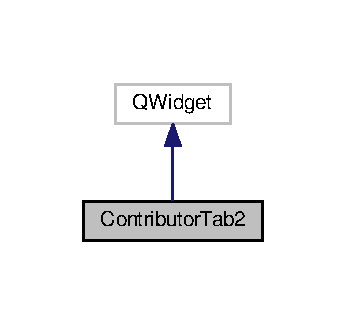
\includegraphics[width=166pt]{classContributorTab2__inherit__graph}
\end{center}
\end{figure}


Collaboration diagram for Contributor\+Tab2\+:\nopagebreak
\begin{figure}[H]
\begin{center}
\leavevmode
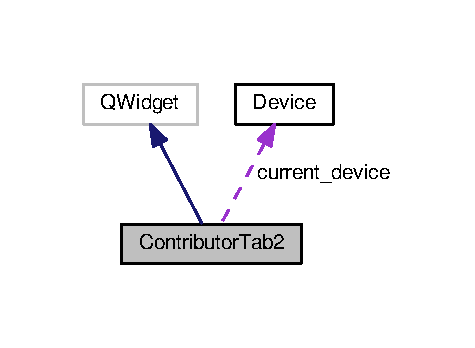
\includegraphics[width=228pt]{classContributorTab2__coll__graph}
\end{center}
\end{figure}
\subsection*{Public Slots}
\begin{DoxyCompactItemize}
\item 
void \hyperlink{classContributorTab2_abf252c3c3cacdc4a4d1f369ffd4fbb99}{update\+Screen} (\hyperlink{classDevice}{Device} device)
\begin{DoxyCompactList}\small\item\em update\+Screen \end{DoxyCompactList}\item 
void \hyperlink{classContributorTab2_a22fb06bbd151a407ff40404897cabb4d}{on\+\_\+description\+\_\+link\+Activated} (const Q\+String \&link)
\begin{DoxyCompactList}\small\item\em \hyperlink{classContributorTab2_a22fb06bbd151a407ff40404897cabb4d}{Contributor\+Tab2\+::on\+\_\+description\+\_\+link\+Activated}. \end{DoxyCompactList}\item 
\mbox{\Hypertarget{classContributorTab2_ab8a868f09884b9b5ce0e4aa7c6940166}\label{classContributorTab2_ab8a868f09884b9b5ce0e4aa7c6940166}} 
void \hyperlink{classContributorTab2_ab8a868f09884b9b5ce0e4aa7c6940166}{receive\+Reboot} ()
\begin{DoxyCompactList}\small\item\em sets reboot button and label to visible when method received. \end{DoxyCompactList}\item 
\mbox{\Hypertarget{classContributorTab2_a3b818b61d87562521615de0b57f29a58}\label{classContributorTab2_a3b818b61d87562521615de0b57f29a58}} 
void \hyperlink{classContributorTab2_a3b818b61d87562521615de0b57f29a58}{Reboot\+Machine} ()
\begin{DoxyCompactList}\small\item\em reboots machine. \end{DoxyCompactList}\end{DoxyCompactItemize}
\subsection*{Public Member Functions}
\begin{DoxyCompactItemize}
\item 
\hyperlink{classContributorTab2_afb63f19687c265fe4fc325040cc2d8d7}{Contributor\+Tab2} (Q\+Widget $\ast$parent=0)
\begin{DoxyCompactList}\small\item\em \hyperlink{classContributorTab2}{Contributor\+Tab2}. \end{DoxyCompactList}\item 
string $\ast$ \hyperlink{classContributorTab2_a5b9c63b5497b9e095624cd01969f0101}{Download\+Info} (string owner\+\_\+git\+\_\+id)
\begin{DoxyCompactList}\small\item\em Download\+Info. \end{DoxyCompactList}\item 
string \hyperlink{classContributorTab2_aed6aceb6bd6c0fb3d32e435a731133d8}{get\+Avatar\+Image} (string url, string owner\+\_\+git\+\_\+id)
\begin{DoxyCompactList}\small\item\em get\+Avatar\+Image \end{DoxyCompactList}\end{DoxyCompactItemize}
\subsection*{Protected Member Functions}
\begin{DoxyCompactItemize}
\item 
void \hyperlink{classContributorTab2_a93c3ed51e9f40c439ed4182e4407434a}{mouse\+Press\+Event} (Q\+Mouse\+Event $\ast$event)
\begin{DoxyCompactList}\small\item\em \hyperlink{classContributorTab2_a93c3ed51e9f40c439ed4182e4407434a}{Contributor\+Tab2\+::mouse\+Press\+Event}. \end{DoxyCompactList}\item 
void \hyperlink{classContributorTab2_a7bc323cf603d03913d96ade9536d8f7e}{clear\+Layout} (Q\+Layout $\ast$layout, bool delete\+Widgets)
\begin{DoxyCompactList}\small\item\em \hyperlink{classConsoleTab_aae70e23b23e401b219edefcac4882eaf}{Console\+Tab\+::clear\+Layout}. \end{DoxyCompactList}\end{DoxyCompactItemize}
\subsection*{Protected Attributes}
\begin{DoxyCompactItemize}
\item 
\mbox{\Hypertarget{classContributorTab2_a7ca94f57e9793023fc331f7245b69975}\label{classContributorTab2_a7ca94f57e9793023fc331f7245b69975}} 
Q\+Label $\ast$ {\bfseries label}
\item 
\mbox{\Hypertarget{classContributorTab2_a759abc114bf3279f38d9a685a80624ab}\label{classContributorTab2_a759abc114bf3279f38d9a685a80624ab}} 
Q\+Label $\ast$ {\bfseries image\+\_\+label}
\item 
\mbox{\Hypertarget{classContributorTab2_aab2a2dcd6d09268e97b19e056cedc1ba}\label{classContributorTab2_aab2a2dcd6d09268e97b19e056cedc1ba}} 
Q\+Label $\ast$ {\bfseries contributor\+\_\+label}
\item 
\mbox{\Hypertarget{classContributorTab2_a146e398d75b803a3594c2266d7e3114e}\label{classContributorTab2_a146e398d75b803a3594c2266d7e3114e}} 
Q\+Label $\ast$ {\bfseries website\+\_\+label}
\item 
\mbox{\Hypertarget{classContributorTab2_a55dc52eeb2ec67b05856f14fe7855c8f}\label{classContributorTab2_a55dc52eeb2ec67b05856f14fe7855c8f}} 
Q\+Label $\ast$ {\bfseries bio\+\_\+label}
\item 
\mbox{\Hypertarget{classContributorTab2_a8c916252a46d0f7885438208e61c39bf}\label{classContributorTab2_a8c916252a46d0f7885438208e61c39bf}} 
Q\+Label $\ast$ {\bfseries email\+\_\+label}
\item 
\mbox{\Hypertarget{classContributorTab2_aaa2f175ef25a9d56f4554486d0d44542}\label{classContributorTab2_aaa2f175ef25a9d56f4554486d0d44542}} 
Q\+Label $\ast$ {\bfseries reboot\+\_\+label}
\item 
\mbox{\Hypertarget{classContributorTab2_a774327038118da4fa33b53a83e37b5ce}\label{classContributorTab2_a774327038118da4fa33b53a83e37b5ce}} 
Q\+Push\+Button $\ast$ {\bfseries reboot\+\_\+button}
\item 
\mbox{\Hypertarget{classContributorTab2_a7acd0fcbd7352b31fda260d343b0511b}\label{classContributorTab2_a7acd0fcbd7352b31fda260d343b0511b}} 
Q\+V\+Box\+Layout $\ast$ {\bfseries main\+Layout}
\item 
\mbox{\Hypertarget{classContributorTab2_a777786adf2c84debc74fe0757c3246b2}\label{classContributorTab2_a777786adf2c84debc74fe0757c3246b2}} 
Q\+Main\+Window $\ast$ {\bfseries main\+Window}
\item 
\mbox{\Hypertarget{classContributorTab2_a42debe86889bf6ae1a45614662690a91}\label{classContributorTab2_a42debe86889bf6ae1a45614662690a91}} 
\hyperlink{classDevice}{Device} {\bfseries current\+\_\+device}
\item 
\mbox{\Hypertarget{classContributorTab2_add3ea333f932475a7eb3a69cdcb5ba48}\label{classContributorTab2_add3ea333f932475a7eb3a69cdcb5ba48}} 
string $\ast$ {\bfseries details}
\end{DoxyCompactItemize}


\subsection{Constructor \& Destructor Documentation}
\mbox{\Hypertarget{classContributorTab2_afb63f19687c265fe4fc325040cc2d8d7}\label{classContributorTab2_afb63f19687c265fe4fc325040cc2d8d7}} 
\index{Contributor\+Tab2@{Contributor\+Tab2}!Contributor\+Tab2@{Contributor\+Tab2}}
\index{Contributor\+Tab2@{Contributor\+Tab2}!Contributor\+Tab2@{Contributor\+Tab2}}
\subsubsection{\texorpdfstring{Contributor\+Tab2()}{ContributorTab2()}}
{\footnotesize\ttfamily Contributor\+Tab2\+::\+Contributor\+Tab2 (\begin{DoxyParamCaption}\item[{Q\+Widget $\ast$}]{parent = {\ttfamily 0} }\end{DoxyParamCaption})}



\hyperlink{classContributorTab2}{Contributor\+Tab2}. 

\hyperlink{classContributorTab2_afb63f19687c265fe4fc325040cc2d8d7}{Contributor\+Tab2\+::\+Contributor\+Tab2}.

Contirbutor tab. 
\begin{DoxyParams}{Parameters}
{\em parent} & \\
\hline
{\em parent} & Contributor tab, dispays information about the contributing devleoper. \\
\hline
\end{DoxyParams}


\subsection{Member Function Documentation}
\mbox{\Hypertarget{classContributorTab2_a7bc323cf603d03913d96ade9536d8f7e}\label{classContributorTab2_a7bc323cf603d03913d96ade9536d8f7e}} 
\index{Contributor\+Tab2@{Contributor\+Tab2}!clear\+Layout@{clear\+Layout}}
\index{clear\+Layout@{clear\+Layout}!Contributor\+Tab2@{Contributor\+Tab2}}
\subsubsection{\texorpdfstring{clear\+Layout()}{clearLayout()}}
{\footnotesize\ttfamily void Contributor\+Tab2\+::clear\+Layout (\begin{DoxyParamCaption}\item[{Q\+Layout $\ast$}]{layout,  }\item[{bool}]{delete\+Widgets = {\ttfamily true} }\end{DoxyParamCaption})\hspace{0.3cm}{\ttfamily [protected]}}



\hyperlink{classConsoleTab_aae70e23b23e401b219edefcac4882eaf}{Console\+Tab\+::clear\+Layout}. 

Clears the layout of the tab. 
\begin{DoxyParams}{Parameters}
{\em layout} & layout to be removed. \\
\hline
{\em delete\+Widgets} & clear widgets as well as layout Clears the layout for future method calls.\\
\hline
{\em layout} & \\
\hline
{\em delete\+Widgets} & Clears the layout for future method calls. \\
\hline
\end{DoxyParams}
\mbox{\Hypertarget{classContributorTab2_a5b9c63b5497b9e095624cd01969f0101}\label{classContributorTab2_a5b9c63b5497b9e095624cd01969f0101}} 
\index{Contributor\+Tab2@{Contributor\+Tab2}!Download\+Info@{Download\+Info}}
\index{Download\+Info@{Download\+Info}!Contributor\+Tab2@{Contributor\+Tab2}}
\subsubsection{\texorpdfstring{Download\+Info()}{DownloadInfo()}}
{\footnotesize\ttfamily string $\ast$ Contributor\+Tab2\+::\+Download\+Info (\begin{DoxyParamCaption}\item[{string}]{owner\+\_\+git\+\_\+id }\end{DoxyParamCaption})}



Download\+Info. 

\hyperlink{classContributorTab2_a5b9c63b5497b9e095624cd01969f0101}{Contributor\+Tab2\+::\+Download\+Info}.

Downloads information of a contributor. 
\begin{DoxyParams}{Parameters}
{\em owner\+\_\+git\+\_\+id} & contributor\textquotesingle{}s user id on github.\+com \\
\hline
\end{DoxyParams}
\begin{DoxyReturn}{Returns}

\end{DoxyReturn}

\begin{DoxyParams}{Parameters}
{\em owner\+\_\+git\+\_\+id} & \\
\hline
\end{DoxyParams}
\begin{DoxyReturn}{Returns}
returns a string array of contributor information downloaded from backend servlet. 
\end{DoxyReturn}
\mbox{\Hypertarget{classContributorTab2_aed6aceb6bd6c0fb3d32e435a731133d8}\label{classContributorTab2_aed6aceb6bd6c0fb3d32e435a731133d8}} 
\index{Contributor\+Tab2@{Contributor\+Tab2}!get\+Avatar\+Image@{get\+Avatar\+Image}}
\index{get\+Avatar\+Image@{get\+Avatar\+Image}!Contributor\+Tab2@{Contributor\+Tab2}}
\subsubsection{\texorpdfstring{get\+Avatar\+Image()}{getAvatarImage()}}
{\footnotesize\ttfamily string Contributor\+Tab2\+::get\+Avatar\+Image (\begin{DoxyParamCaption}\item[{string}]{url,  }\item[{string}]{owner\+\_\+git\+\_\+id }\end{DoxyParamCaption})}



get\+Avatar\+Image 

\hyperlink{classContributorTab2_aed6aceb6bd6c0fb3d32e435a731133d8}{Contributor\+Tab2\+::get\+Avatar\+Image}.

Gets the github avatar of a contibutor. 
\begin{DoxyParams}{Parameters}
{\em url} & gtihub.\+com url to get avatar from \\
\hline
{\em owner\+\_\+git\+\_\+id} & \\
\hline
\end{DoxyParams}
\begin{DoxyReturn}{Returns}

\end{DoxyReturn}

\begin{DoxyParams}{Parameters}
{\em url} & \\
\hline
{\em owner\+\_\+git\+\_\+id} & \\
\hline
\end{DoxyParams}
\begin{DoxyReturn}{Returns}
downloads contributor\textquotesingle{}s avatar image from github\textquotesingle{}s url 
\end{DoxyReturn}
\mbox{\Hypertarget{classContributorTab2_a93c3ed51e9f40c439ed4182e4407434a}\label{classContributorTab2_a93c3ed51e9f40c439ed4182e4407434a}} 
\index{Contributor\+Tab2@{Contributor\+Tab2}!mouse\+Press\+Event@{mouse\+Press\+Event}}
\index{mouse\+Press\+Event@{mouse\+Press\+Event}!Contributor\+Tab2@{Contributor\+Tab2}}
\subsubsection{\texorpdfstring{mouse\+Press\+Event()}{mousePressEvent()}}
{\footnotesize\ttfamily void Contributor\+Tab2\+::mouse\+Press\+Event (\begin{DoxyParamCaption}\item[{Q\+Mouse\+Event $\ast$}]{event }\end{DoxyParamCaption})\hspace{0.3cm}{\ttfamily [protected]}}



\hyperlink{classContributorTab2_a93c3ed51e9f40c439ed4182e4407434a}{Contributor\+Tab2\+::mouse\+Press\+Event}. 


\begin{DoxyParams}{Parameters}
{\em event} & sends a message to \hyperlink{classGetOS}{Get\+OS} to open contributors webpage when label clicked. \\
\hline
\end{DoxyParams}
\mbox{\Hypertarget{classContributorTab2_a22fb06bbd151a407ff40404897cabb4d}\label{classContributorTab2_a22fb06bbd151a407ff40404897cabb4d}} 
\index{Contributor\+Tab2@{Contributor\+Tab2}!on\+\_\+description\+\_\+link\+Activated@{on\+\_\+description\+\_\+link\+Activated}}
\index{on\+\_\+description\+\_\+link\+Activated@{on\+\_\+description\+\_\+link\+Activated}!Contributor\+Tab2@{Contributor\+Tab2}}
\subsubsection{\texorpdfstring{on\+\_\+description\+\_\+link\+Activated}{on\_description\_linkActivated}}
{\footnotesize\ttfamily void Contributor\+Tab2\+::on\+\_\+description\+\_\+link\+Activated (\begin{DoxyParamCaption}\item[{const Q\+String \&}]{link }\end{DoxyParamCaption})\hspace{0.3cm}{\ttfamily [slot]}}



\hyperlink{classContributorTab2_a22fb06bbd151a407ff40404897cabb4d}{Contributor\+Tab2\+::on\+\_\+description\+\_\+link\+Activated}. 

sends a message to \hyperlink{classGetOS}{Get\+OS} to send email to contributor when label clicked. 
\begin{DoxyParams}{Parameters}
{\em link} & email link to be launched in mail client. \\
\hline
\end{DoxyParams}
\mbox{\Hypertarget{classContributorTab2_abf252c3c3cacdc4a4d1f369ffd4fbb99}\label{classContributorTab2_abf252c3c3cacdc4a4d1f369ffd4fbb99}} 
\index{Contributor\+Tab2@{Contributor\+Tab2}!update\+Screen@{update\+Screen}}
\index{update\+Screen@{update\+Screen}!Contributor\+Tab2@{Contributor\+Tab2}}
\subsubsection{\texorpdfstring{update\+Screen}{updateScreen}}
{\footnotesize\ttfamily void Contributor\+Tab2\+::update\+Screen (\begin{DoxyParamCaption}\item[{\hyperlink{classDevice}{Device}}]{device }\end{DoxyParamCaption})\hspace{0.3cm}{\ttfamily [slot]}}



update\+Screen 

\hyperlink{classContributorTab2_abf252c3c3cacdc4a4d1f369ffd4fbb99}{Contributor\+Tab2\+::update\+Screen}.

Updates the screen with the contributor details as found in the \hyperlink{classDevice}{Device} object. 
\begin{DoxyParams}{Parameters}
{\em device} & \\
\hline
{\em device} & updates the contributor tab with information on a specific developer. Information derived from device object. \\
\hline
\end{DoxyParams}


The documentation for this class was generated from the following files\+:\begin{DoxyCompactItemize}
\item 
Contributor\+Tab2.\+h\item 
Contributor\+Tab2.\+cpp\end{DoxyCompactItemize}

\hypertarget{classDevice}{}\section{Device Class Reference}
\label{classDevice}\index{Device@{Device}}
\subsection*{Public Member Functions}
\begin{DoxyCompactItemize}
\item 
\hyperlink{classDevice_a64ba12dcc5f4267486c5d545d04dcf68}{Device} ()
\begin{DoxyCompactList}\small\item\em \hyperlink{classDevice}{Device}. \end{DoxyCompactList}\item 
\hyperlink{classDevice_a107e7a95a02edc5ff586dfc831f1eb76}{Device} (string id, string description, string name, string modulename)
\begin{DoxyCompactList}\small\item\em \hyperlink{classDevice}{Device}. \end{DoxyCompactList}\item 
\hyperlink{classDevice_a11aa3e7c780559e7749bea3ac702e55e}{Device} (string m\+\_\+id, string m\+\_\+description, bool is\+Installed, bool is\+Failed, string success\+\_\+code, string status)
\begin{DoxyCompactList}\small\item\em \hyperlink{classDevice}{Device}. \end{DoxyCompactList}\item 
string \hyperlink{classDevice_a0c77b871987e94ec9088e8ab78f27293}{parse\+Device\+Id} (string device\+\_\+id)
\item 
bool \hyperlink{classDevice_acd077de5b2954ce456927e021c5de5df}{operator$<$} (const \hyperlink{classDevice}{Device} rhs) const
\begin{DoxyCompactList}\small\item\em operator $<$ \end{DoxyCompactList}\item 
bool \hyperlink{classDevice_a660d5da7a710da202ac6c58766370283}{operator$<$} (const \hyperlink{classDevice}{Device} rhs)
\begin{DoxyCompactList}\small\item\em operator $<$ \end{DoxyCompactList}\item 
bool \hyperlink{classDevice_a1078839b751f8366b5170d4daefa26b4}{is\+Upgradeable} ()
\begin{DoxyCompactList}\small\item\em is\+Upgradeable \end{DoxyCompactList}\item 
string \hyperlink{classDevice_abdadd7bc6fa1760aeaa9f87dd2f96f59}{get\+Installed\+Status} ()
\begin{DoxyCompactList}\small\item\em get\+Installed\+Status \end{DoxyCompactList}\item 
\hyperlink{classDevice}{Device} \hyperlink{classDevice_a2036c2bc77979808046f7ecae94ec602}{getinfo} ()
\begin{DoxyCompactList}\small\item\em getinfo \end{DoxyCompactList}\item 
const std\+::string \& \hyperlink{classDevice_ae5b04fdd1bf82d2dba2ec249e92e4da5}{get\+Commit} () const
\begin{DoxyCompactList}\small\item\em get\+Commit \end{DoxyCompactList}\item 
void \hyperlink{classDevice_a2d549bad1c70b5768698dbc2175669ef}{set\+Commit} (const std\+::string \&commit)
\begin{DoxyCompactList}\small\item\em set\+Commit \end{DoxyCompactList}\item 
const std\+::string \& \hyperlink{classDevice_a6ba1792dd4f33f99e7b3ff97c4fae153}{get\+Description} () const
\begin{DoxyCompactList}\small\item\em get\+Description \end{DoxyCompactList}\item 
void \hyperlink{classDevice_a3f71228960ac3bfca0a1cca254ea782b}{set\+Description} (const std\+::string \&description)
\begin{DoxyCompactList}\small\item\em set\+Description \end{DoxyCompactList}\item 
const std\+::string \& \hyperlink{classDevice_ace938c6c2efffdcc2d17d49440cb55b7}{get\+Deviceid} () const
\begin{DoxyCompactList}\small\item\em get\+Deviceid \end{DoxyCompactList}\item 
void \hyperlink{classDevice_a8bd16b3e099e864db3c09ba4f6225fb0}{set\+Deviceid} (const std\+::string \&deviceid)
\begin{DoxyCompactList}\small\item\em set\+Deviceid \end{DoxyCompactList}\item 
const std\+::string \& \hyperlink{classDevice_a96f94097331f294afc73c6358918d408}{get\+Git\+Url} () const
\begin{DoxyCompactList}\small\item\em get\+Git\+Url \end{DoxyCompactList}\item 
void \hyperlink{classDevice_ae8587aa062a7a2f2b5b77e9a15569e53}{set\+Git\+Url} (const std\+::string \&git\+Url)
\begin{DoxyCompactList}\small\item\em set\+Git\+Url \end{DoxyCompactList}\item 
const std\+::string \& \hyperlink{classDevice_a77eeec87fea2ffc4d4140b315613bb1b}{get\+Modulename} () const
\begin{DoxyCompactList}\small\item\em get\+Modulename \end{DoxyCompactList}\item 
void \hyperlink{classDevice_a09e9d9bbcfa76268b7ebc30afa680c69}{set\+Modulename} (const std\+::string \&modulename)
\begin{DoxyCompactList}\small\item\em set\+Modulename \end{DoxyCompactList}\item 
const std\+::string \& \hyperlink{classDevice_a2b4556e5a3b1f955c3e498e1de75051c}{get\+Owner\+Git\+Id} () const
\begin{DoxyCompactList}\small\item\em get\+Owner\+Git\+Id \end{DoxyCompactList}\item 
void \hyperlink{classDevice_aabc16749d0fe22ec25ca525fbd2b9dc2}{set\+Owner\+Git\+Id} (const std\+::string \&owner\+Git\+Id)
\begin{DoxyCompactList}\small\item\em set\+Owner\+Git\+Id \end{DoxyCompactList}\item 
const std\+::string \& \hyperlink{classDevice_a19c62e8fa746efc12e6c0521b690bf03}{get\+Success\+Code} () const
\begin{DoxyCompactList}\small\item\em get\+Success\+Code \end{DoxyCompactList}\item 
void \hyperlink{classDevice_ae70b727a6230454baccc6da6cfd819a7}{set\+Success\+Code} (const std\+::string \&success\+Code)
\begin{DoxyCompactList}\small\item\em set\+Success\+Code \end{DoxyCompactList}\item 
const std\+::string \& \hyperlink{classDevice_a7c1221950b9ec064b023c4033454774a}{get\+Devicename} () const
\begin{DoxyCompactList}\small\item\em get\+Devicename \end{DoxyCompactList}\item 
void \hyperlink{classDevice_ad1f6005dcab32855477814fa9533315d}{set\+Devicename} (const std\+::string \&devicename)
\begin{DoxyCompactList}\small\item\em set\+Devicename \end{DoxyCompactList}\item 
const std\+::string \& \hyperlink{classDevice_a3c0a93766217f57848cf6871aeb9ffc2}{get\+Set\+Command} () const
\begin{DoxyCompactList}\small\item\em get\+Set\+Command \end{DoxyCompactList}\item 
void \hyperlink{classDevice_afad48633a288b303f88f7d607c64cca3}{set\+Set\+Command} (const std\+::string \&set\+Command)
\begin{DoxyCompactList}\small\item\em set\+Set\+Command \end{DoxyCompactList}\item 
const int \& \hyperlink{classDevice_abbf7d73cde4dc08996414956fc25188d}{get\+Vote\+Difference} () const
\begin{DoxyCompactList}\small\item\em get\+Vote\+Difference \end{DoxyCompactList}\item 
void \hyperlink{classDevice_acf378aa086771dd7c64626abb8a74821}{set\+Vote\+Difference} (const int \&vote\+Difference)
\begin{DoxyCompactList}\small\item\em set\+Vote\+Difference \end{DoxyCompactList}\item 
const bool \hyperlink{classDevice_a068c25d48712783fd0dc759d4505c615}{get\+Attempted\+Install} () const
\begin{DoxyCompactList}\small\item\em get\+Attempted\+Install \end{DoxyCompactList}\item 
void \hyperlink{classDevice_af2591540bf77d38b8e4c09b90e8dfaba}{set\+Attempted\+Install} (bool installed)
\begin{DoxyCompactList}\small\item\em set\+Attempted\+Install \end{DoxyCompactList}\item 
const string \& \hyperlink{classDevice_ad49afa64f231ac899736cc21027766f2}{get\+Status} () const
\begin{DoxyCompactList}\small\item\em get\+Status \end{DoxyCompactList}\item 
void \hyperlink{classDevice_a46b5e30da5b43b09c0785a054bfb678a}{set\+Status} (const string \&status)
\begin{DoxyCompactList}\small\item\em set\+Status \end{DoxyCompactList}\item 
bool \hyperlink{classDevice_afe6f638cc2bcc512f5bc1f2fef39fe88}{is\+Is\+Upgradeable} () const
\begin{DoxyCompactList}\small\item\em is\+Is\+Upgradeable \end{DoxyCompactList}\item 
void \hyperlink{classDevice_a3b5d4af66cacd8e1b0e45219c16ee084}{set\+Is\+Upgradeable} (bool \hyperlink{classDevice_a1078839b751f8366b5170d4daefa26b4}{is\+Upgradeable})
\begin{DoxyCompactList}\small\item\em set\+Is\+Upgradeable \end{DoxyCompactList}\item 
bool \hyperlink{classDevice_a697feb57b759c13cb1b56f004e61229b}{is\+Is\+Installed} () const
\begin{DoxyCompactList}\small\item\em is\+Is\+Installed \end{DoxyCompactList}\item 
void \hyperlink{classDevice_aec222a879b4a9aadd1a083a7aff2e516}{set\+Is\+Installed} (bool is\+Installed)
\begin{DoxyCompactList}\small\item\em set\+Is\+Installed \end{DoxyCompactList}\item 
void \hyperlink{classDevice_a15d7c755aed944da8514902d06d21ea9}{set\+Apt\+Installed} (bool apt\+\_\+install)
\begin{DoxyCompactList}\small\item\em set\+Apt\+Installed \end{DoxyCompactList}\item 
bool \hyperlink{classDevice_a2ea735319a841af580e6ada8ab3b4076}{get\+Apt\+Installed} ()
\begin{DoxyCompactList}\small\item\em get\+Apt\+Installed \end{DoxyCompactList}\end{DoxyCompactItemize}
\subsection*{Public Attributes}
\begin{DoxyCompactItemize}
\item 
\mbox{\Hypertarget{classDevice_a1eb16134b02676dd87524745e70aa439}\label{classDevice_a1eb16134b02676dd87524745e70aa439}} 
std\+::string {\bfseries deviceid}
\item 
\mbox{\Hypertarget{classDevice_a306ead055a0bfe68d4dbc947d1176cad}\label{classDevice_a306ead055a0bfe68d4dbc947d1176cad}} 
std\+::string {\bfseries modulename}
\item 
\mbox{\Hypertarget{classDevice_a5660725c3c3d2349a3b164e89d27a401}\label{classDevice_a5660725c3c3d2349a3b164e89d27a401}} 
std\+::string {\bfseries description}
\item 
\mbox{\Hypertarget{classDevice_ac379e1898eb7d56f85efc2aca209a508}\label{classDevice_ac379e1898eb7d56f85efc2aca209a508}} 
std\+::string {\bfseries commit}
\item 
\mbox{\Hypertarget{classDevice_ae95f052236ec631403484833f5b1e618}\label{classDevice_ae95f052236ec631403484833f5b1e618}} 
std\+::string {\bfseries git\+\_\+url}
\item 
\mbox{\Hypertarget{classDevice_a0ac795464def7d9466de72c954fdeac1}\label{classDevice_a0ac795464def7d9466de72c954fdeac1}} 
std\+::string {\bfseries success\+\_\+code}
\item 
\mbox{\Hypertarget{classDevice_a26f60bd0aef8477a9522b018583fd020}\label{classDevice_a26f60bd0aef8477a9522b018583fd020}} 
std\+::string {\bfseries owner\+\_\+git\+\_\+id}
\item 
\mbox{\Hypertarget{classDevice_aeb1dfe30b1ee923134098b7e0693d629}\label{classDevice_aeb1dfe30b1ee923134098b7e0693d629}} 
std\+::string {\bfseries devicename}
\item 
\mbox{\Hypertarget{classDevice_a2decbd2aba65213d36c6aafe9a68680d}\label{classDevice_a2decbd2aba65213d36c6aafe9a68680d}} 
std\+::string {\bfseries set\+Command}
\item 
\mbox{\Hypertarget{classDevice_a3ff73d2c41d11d87b9681f151ad80cc2}\label{classDevice_a3ff73d2c41d11d87b9681f151ad80cc2}} 
bool {\bfseries Apt\+Installed}
\item 
\mbox{\Hypertarget{classDevice_a7f20acfc3fbc1ea6da416b64223d69a1}\label{classDevice_a7f20acfc3fbc1ea6da416b64223d69a1}} 
bool {\bfseries attempted\+\_\+install}
\item 
\mbox{\Hypertarget{classDevice_a26bbc09d2ff3c76f660463c8438df083}\label{classDevice_a26bbc09d2ff3c76f660463c8438df083}} 
int {\bfseries vote\+\_\+difference}
\item 
\mbox{\Hypertarget{classDevice_a1ab968c173c863b0ceccb7418c0a281c}\label{classDevice_a1ab968c173c863b0ceccb7418c0a281c}} 
bool {\bfseries is\+\_\+upgradeable}
\item 
\mbox{\Hypertarget{classDevice_ad62a2bdc698beba3b477a587afaeb1f3}\label{classDevice_ad62a2bdc698beba3b477a587afaeb1f3}} 
bool {\bfseries is\+\_\+installed}
\item 
\mbox{\Hypertarget{classDevice_ad3cd9d9d8054a8ef1a136ded17d2fff7}\label{classDevice_ad3cd9d9d8054a8ef1a136ded17d2fff7}} 
string {\bfseries status}
\end{DoxyCompactItemize}


\subsection{Constructor \& Destructor Documentation}
\mbox{\Hypertarget{classDevice_a64ba12dcc5f4267486c5d545d04dcf68}\label{classDevice_a64ba12dcc5f4267486c5d545d04dcf68}} 
\index{Device@{Device}!Device@{Device}}
\index{Device@{Device}!Device@{Device}}
\subsubsection{\texorpdfstring{Device()}{Device()}\hspace{0.1cm}{\footnotesize\ttfamily [1/3]}}
{\footnotesize\ttfamily Device\+::\+Device (\begin{DoxyParamCaption}{ }\end{DoxyParamCaption})}



\hyperlink{classDevice}{Device}. 

Default constructor. \mbox{\Hypertarget{classDevice_a107e7a95a02edc5ff586dfc831f1eb76}\label{classDevice_a107e7a95a02edc5ff586dfc831f1eb76}} 
\index{Device@{Device}!Device@{Device}}
\index{Device@{Device}!Device@{Device}}
\subsubsection{\texorpdfstring{Device()}{Device()}\hspace{0.1cm}{\footnotesize\ttfamily [2/3]}}
{\footnotesize\ttfamily Device\+::\+Device (\begin{DoxyParamCaption}\item[{string}]{id,  }\item[{string}]{description,  }\item[{string}]{name,  }\item[{string}]{modulename }\end{DoxyParamCaption})}



\hyperlink{classDevice}{Device}. 

Constructor as used in downloading remote configuration. 
\begin{DoxyParams}{Parameters}
{\em id} & \\
\hline
{\em description} & \\
\hline
{\em name} & \\
\hline
{\em modulename} & \\
\hline
\end{DoxyParams}
\mbox{\Hypertarget{classDevice_a11aa3e7c780559e7749bea3ac702e55e}\label{classDevice_a11aa3e7c780559e7749bea3ac702e55e}} 
\index{Device@{Device}!Device@{Device}}
\index{Device@{Device}!Device@{Device}}
\subsubsection{\texorpdfstring{Device()}{Device()}\hspace{0.1cm}{\footnotesize\ttfamily [3/3]}}
{\footnotesize\ttfamily Device\+::\+Device (\begin{DoxyParamCaption}\item[{string}]{m\+\_\+id,  }\item[{string}]{m\+\_\+description,  }\item[{bool}]{is\+Installed,  }\item[{bool}]{is\+Failed,  }\item[{string}]{success\+\_\+code,  }\item[{string}]{status }\end{DoxyParamCaption})}



\hyperlink{classDevice}{Device}. 

Constructor as used when obtaining information from history file. 
\begin{DoxyParams}{Parameters}
{\em m\+\_\+id} & \\
\hline
{\em m\+\_\+description} & \\
\hline
{\em is\+Installed} & \\
\hline
{\em is\+Failed} & \\
\hline
{\em success\+\_\+code} & \\
\hline
{\em status} & \\
\hline
\end{DoxyParams}


\subsection{Member Function Documentation}
\mbox{\Hypertarget{classDevice_a2ea735319a841af580e6ada8ab3b4076}\label{classDevice_a2ea735319a841af580e6ada8ab3b4076}} 
\index{Device@{Device}!get\+Apt\+Installed@{get\+Apt\+Installed}}
\index{get\+Apt\+Installed@{get\+Apt\+Installed}!Device@{Device}}
\subsubsection{\texorpdfstring{get\+Apt\+Installed()}{getAptInstalled()}}
{\footnotesize\ttfamily bool Device\+::get\+Apt\+Installed (\begin{DoxyParamCaption}{ }\end{DoxyParamCaption})}



get\+Apt\+Installed 

Returns true if packages were installed using apt-\/undo. \begin{DoxyReturn}{Returns}

\end{DoxyReturn}
\mbox{\Hypertarget{classDevice_a068c25d48712783fd0dc759d4505c615}\label{classDevice_a068c25d48712783fd0dc759d4505c615}} 
\index{Device@{Device}!get\+Attempted\+Install@{get\+Attempted\+Install}}
\index{get\+Attempted\+Install@{get\+Attempted\+Install}!Device@{Device}}
\subsubsection{\texorpdfstring{get\+Attempted\+Install()}{getAttemptedInstall()}}
{\footnotesize\ttfamily const bool Device\+::get\+Attempted\+Install (\begin{DoxyParamCaption}{ }\end{DoxyParamCaption}) const}



get\+Attempted\+Install 

returns true if an attempred install of the device has been made. \begin{DoxyReturn}{Returns}

\end{DoxyReturn}
\mbox{\Hypertarget{classDevice_ae5b04fdd1bf82d2dba2ec249e92e4da5}\label{classDevice_ae5b04fdd1bf82d2dba2ec249e92e4da5}} 
\index{Device@{Device}!get\+Commit@{get\+Commit}}
\index{get\+Commit@{get\+Commit}!Device@{Device}}
\subsubsection{\texorpdfstring{get\+Commit()}{getCommit()}}
{\footnotesize\ttfamily const std\+::string \& Device\+::get\+Commit (\begin{DoxyParamCaption}{ }\end{DoxyParamCaption}) const}



get\+Commit 

Returns commit hash. \begin{DoxyReturn}{Returns}

\end{DoxyReturn}
\mbox{\Hypertarget{classDevice_a6ba1792dd4f33f99e7b3ff97c4fae153}\label{classDevice_a6ba1792dd4f33f99e7b3ff97c4fae153}} 
\index{Device@{Device}!get\+Description@{get\+Description}}
\index{get\+Description@{get\+Description}!Device@{Device}}
\subsubsection{\texorpdfstring{get\+Description()}{getDescription()}}
{\footnotesize\ttfamily const std\+::string \& Device\+::get\+Description (\begin{DoxyParamCaption}{ }\end{DoxyParamCaption}) const}



get\+Description 

returns device description as found locally.. \begin{DoxyReturn}{Returns}

\end{DoxyReturn}
\mbox{\Hypertarget{classDevice_ace938c6c2efffdcc2d17d49440cb55b7}\label{classDevice_ace938c6c2efffdcc2d17d49440cb55b7}} 
\index{Device@{Device}!get\+Deviceid@{get\+Deviceid}}
\index{get\+Deviceid@{get\+Deviceid}!Device@{Device}}
\subsubsection{\texorpdfstring{get\+Deviceid()}{getDeviceid()}}
{\footnotesize\ttfamily const std\+::string \& Device\+::get\+Deviceid (\begin{DoxyParamCaption}{ }\end{DoxyParamCaption}) const}



get\+Deviceid 

returns device id. \begin{DoxyReturn}{Returns}

\end{DoxyReturn}
\mbox{\Hypertarget{classDevice_a7c1221950b9ec064b023c4033454774a}\label{classDevice_a7c1221950b9ec064b023c4033454774a}} 
\index{Device@{Device}!get\+Devicename@{get\+Devicename}}
\index{get\+Devicename@{get\+Devicename}!Device@{Device}}
\subsubsection{\texorpdfstring{get\+Devicename()}{getDevicename()}}
{\footnotesize\ttfamily const std\+::string \& Device\+::get\+Devicename (\begin{DoxyParamCaption}{ }\end{DoxyParamCaption}) const}



get\+Devicename 

reutrns device name as found on local system. \begin{DoxyReturn}{Returns}

\end{DoxyReturn}
\mbox{\Hypertarget{classDevice_a96f94097331f294afc73c6358918d408}\label{classDevice_a96f94097331f294afc73c6358918d408}} 
\index{Device@{Device}!get\+Git\+Url@{get\+Git\+Url}}
\index{get\+Git\+Url@{get\+Git\+Url}!Device@{Device}}
\subsubsection{\texorpdfstring{get\+Git\+Url()}{getGitUrl()}}
{\footnotesize\ttfamily const std\+::string \& Device\+::get\+Git\+Url (\begin{DoxyParamCaption}{ }\end{DoxyParamCaption}) const}



get\+Git\+Url 

returns device\textquotesingle{}s remote repository url. \begin{DoxyReturn}{Returns}

\end{DoxyReturn}
\mbox{\Hypertarget{classDevice_a2036c2bc77979808046f7ecae94ec602}\label{classDevice_a2036c2bc77979808046f7ecae94ec602}} 
\index{Device@{Device}!getinfo@{getinfo}}
\index{getinfo@{getinfo}!Device@{Device}}
\subsubsection{\texorpdfstring{getinfo()}{getinfo()}}
{\footnotesize\ttfamily \hyperlink{classDevice}{Device} Device\+::getinfo (\begin{DoxyParamCaption}{ }\end{DoxyParamCaption})}



getinfo 

Returns device object. \begin{DoxyReturn}{Returns}

\end{DoxyReturn}
\mbox{\Hypertarget{classDevice_abdadd7bc6fa1760aeaa9f87dd2f96f59}\label{classDevice_abdadd7bc6fa1760aeaa9f87dd2f96f59}} 
\index{Device@{Device}!get\+Installed\+Status@{get\+Installed\+Status}}
\index{get\+Installed\+Status@{get\+Installed\+Status}!Device@{Device}}
\subsubsection{\texorpdfstring{get\+Installed\+Status()}{getInstalledStatus()}}
{\footnotesize\ttfamily string Device\+::get\+Installed\+Status (\begin{DoxyParamCaption}{ }\end{DoxyParamCaption})}



get\+Installed\+Status 

returns install status as found in history file. \begin{DoxyReturn}{Returns}

\end{DoxyReturn}
\mbox{\Hypertarget{classDevice_a77eeec87fea2ffc4d4140b315613bb1b}\label{classDevice_a77eeec87fea2ffc4d4140b315613bb1b}} 
\index{Device@{Device}!get\+Modulename@{get\+Modulename}}
\index{get\+Modulename@{get\+Modulename}!Device@{Device}}
\subsubsection{\texorpdfstring{get\+Modulename()}{getModulename()}}
{\footnotesize\ttfamily const std\+::string \& Device\+::get\+Modulename (\begin{DoxyParamCaption}{ }\end{DoxyParamCaption}) const}



get\+Modulename 

returns module name as defined in tuxconfig file in repository. \begin{DoxyReturn}{Returns}

\end{DoxyReturn}
\mbox{\Hypertarget{classDevice_a2b4556e5a3b1f955c3e498e1de75051c}\label{classDevice_a2b4556e5a3b1f955c3e498e1de75051c}} 
\index{Device@{Device}!get\+Owner\+Git\+Id@{get\+Owner\+Git\+Id}}
\index{get\+Owner\+Git\+Id@{get\+Owner\+Git\+Id}!Device@{Device}}
\subsubsection{\texorpdfstring{get\+Owner\+Git\+Id()}{getOwnerGitId()}}
{\footnotesize\ttfamily const std\+::string \& Device\+::get\+Owner\+Git\+Id (\begin{DoxyParamCaption}{ }\end{DoxyParamCaption}) const}



get\+Owner\+Git\+Id 

returns contibutors github.\+com user id. \begin{DoxyReturn}{Returns}

\end{DoxyReturn}
\mbox{\Hypertarget{classDevice_a3c0a93766217f57848cf6871aeb9ffc2}\label{classDevice_a3c0a93766217f57848cf6871aeb9ffc2}} 
\index{Device@{Device}!get\+Set\+Command@{get\+Set\+Command}}
\index{get\+Set\+Command@{get\+Set\+Command}!Device@{Device}}
\subsubsection{\texorpdfstring{get\+Set\+Command()}{getSetCommand()}}
{\footnotesize\ttfamily const std\+::string \& Device\+::get\+Set\+Command (\begin{DoxyParamCaption}{ }\end{DoxyParamCaption}) const}



get\+Set\+Command 

Not used. \begin{DoxyReturn}{Returns}

\end{DoxyReturn}
\mbox{\Hypertarget{classDevice_ad49afa64f231ac899736cc21027766f2}\label{classDevice_ad49afa64f231ac899736cc21027766f2}} 
\index{Device@{Device}!get\+Status@{get\+Status}}
\index{get\+Status@{get\+Status}!Device@{Device}}
\subsubsection{\texorpdfstring{get\+Status()}{getStatus()}}
{\footnotesize\ttfamily const string \& Device\+::get\+Status (\begin{DoxyParamCaption}{ }\end{DoxyParamCaption}) const}



get\+Status 

Returns device install status as found in history. \begin{DoxyReturn}{Returns}

\end{DoxyReturn}
\mbox{\Hypertarget{classDevice_a19c62e8fa746efc12e6c0521b690bf03}\label{classDevice_a19c62e8fa746efc12e6c0521b690bf03}} 
\index{Device@{Device}!get\+Success\+Code@{get\+Success\+Code}}
\index{get\+Success\+Code@{get\+Success\+Code}!Device@{Device}}
\subsubsection{\texorpdfstring{get\+Success\+Code()}{getSuccessCode()}}
{\footnotesize\ttfamily const std\+::string \& Device\+::get\+Success\+Code (\begin{DoxyParamCaption}{ }\end{DoxyParamCaption}) const}



get\+Success\+Code 

returns success code of a particular installation as defined in backend database. \begin{DoxyReturn}{Returns}

\end{DoxyReturn}
\mbox{\Hypertarget{classDevice_abbf7d73cde4dc08996414956fc25188d}\label{classDevice_abbf7d73cde4dc08996414956fc25188d}} 
\index{Device@{Device}!get\+Vote\+Difference@{get\+Vote\+Difference}}
\index{get\+Vote\+Difference@{get\+Vote\+Difference}!Device@{Device}}
\subsubsection{\texorpdfstring{get\+Vote\+Difference()}{getVoteDifference()}}
{\footnotesize\ttfamily const int \& Device\+::get\+Vote\+Difference (\begin{DoxyParamCaption}{ }\end{DoxyParamCaption}) const}



get\+Vote\+Difference 

Returns the success of the device\textquotesingle{}s install as downloaded. \begin{DoxyReturn}{Returns}

\end{DoxyReturn}
\mbox{\Hypertarget{classDevice_a697feb57b759c13cb1b56f004e61229b}\label{classDevice_a697feb57b759c13cb1b56f004e61229b}} 
\index{Device@{Device}!is\+Is\+Installed@{is\+Is\+Installed}}
\index{is\+Is\+Installed@{is\+Is\+Installed}!Device@{Device}}
\subsubsection{\texorpdfstring{is\+Is\+Installed()}{isIsInstalled()}}
{\footnotesize\ttfamily bool Device\+::is\+Is\+Installed (\begin{DoxyParamCaption}{ }\end{DoxyParamCaption}) const\hspace{0.3cm}{\ttfamily [inline]}}



is\+Is\+Installed 

Returns true if device is installed. \begin{DoxyReturn}{Returns}

\end{DoxyReturn}
\mbox{\Hypertarget{classDevice_afe6f638cc2bcc512f5bc1f2fef39fe88}\label{classDevice_afe6f638cc2bcc512f5bc1f2fef39fe88}} 
\index{Device@{Device}!is\+Is\+Upgradeable@{is\+Is\+Upgradeable}}
\index{is\+Is\+Upgradeable@{is\+Is\+Upgradeable}!Device@{Device}}
\subsubsection{\texorpdfstring{is\+Is\+Upgradeable()}{isIsUpgradeable()}}
{\footnotesize\ttfamily bool Device\+::is\+Is\+Upgradeable (\begin{DoxyParamCaption}{ }\end{DoxyParamCaption}) const\hspace{0.3cm}{\ttfamily [inline]}}



is\+Is\+Upgradeable 

returns true if vote count of device is less than that of remote verison. \begin{DoxyReturn}{Returns}

\end{DoxyReturn}
\mbox{\Hypertarget{classDevice_a1078839b751f8366b5170d4daefa26b4}\label{classDevice_a1078839b751f8366b5170d4daefa26b4}} 
\index{Device@{Device}!is\+Upgradeable@{is\+Upgradeable}}
\index{is\+Upgradeable@{is\+Upgradeable}!Device@{Device}}
\subsubsection{\texorpdfstring{is\+Upgradeable()}{isUpgradeable()}}
{\footnotesize\ttfamily bool Device\+::is\+Upgradeable (\begin{DoxyParamCaption}{ }\end{DoxyParamCaption})}



is\+Upgradeable 

returns true if upgradeable.

Returns true if vote count less than in database. \begin{DoxyReturn}{Returns}

\end{DoxyReturn}
\mbox{\Hypertarget{classDevice_acd077de5b2954ce456927e021c5de5df}\label{classDevice_acd077de5b2954ce456927e021c5de5df}} 
\index{Device@{Device}!operator$<$@{operator$<$}}
\index{operator$<$@{operator$<$}!Device@{Device}}
\subsubsection{\texorpdfstring{operator$<$()}{operator<()}\hspace{0.1cm}{\footnotesize\ttfamily [1/2]}}
{\footnotesize\ttfamily bool Device\+::operator$<$ (\begin{DoxyParamCaption}\item[{const \hyperlink{classDevice}{Device}}]{rhs }\end{DoxyParamCaption}) const}



operator $<$ 

Sorts items when referred by hashmap (const). 
\begin{DoxyParams}{Parameters}
{\em rhs} & \\
\hline
\end{DoxyParams}
\begin{DoxyReturn}{Returns}

\end{DoxyReturn}
\mbox{\Hypertarget{classDevice_a660d5da7a710da202ac6c58766370283}\label{classDevice_a660d5da7a710da202ac6c58766370283}} 
\index{Device@{Device}!operator$<$@{operator$<$}}
\index{operator$<$@{operator$<$}!Device@{Device}}
\subsubsection{\texorpdfstring{operator$<$()}{operator<()}\hspace{0.1cm}{\footnotesize\ttfamily [2/2]}}
{\footnotesize\ttfamily bool Device\+::operator$<$ (\begin{DoxyParamCaption}\item[{const \hyperlink{classDevice}{Device}}]{rhs }\end{DoxyParamCaption})}



operator $<$ 

Sorts items when referred by hashmap 
\begin{DoxyParams}{Parameters}
{\em rhs} & \\
\hline
\end{DoxyParams}
\begin{DoxyReturn}{Returns}

\end{DoxyReturn}
\mbox{\Hypertarget{classDevice_a0c77b871987e94ec9088e8ab78f27293}\label{classDevice_a0c77b871987e94ec9088e8ab78f27293}} 
\index{Device@{Device}!parse\+Device\+Id@{parse\+Device\+Id}}
\index{parse\+Device\+Id@{parse\+Device\+Id}!Device@{Device}}
\subsubsection{\texorpdfstring{parse\+Device\+Id()}{parseDeviceId()}}
{\footnotesize\ttfamily string Device\+::parse\+Device\+Id (\begin{DoxyParamCaption}\item[{string}]{device\+\_\+id }\end{DoxyParamCaption})}

Parses device id to match that of databse \mbox{\Hypertarget{classDevice_a15d7c755aed944da8514902d06d21ea9}\label{classDevice_a15d7c755aed944da8514902d06d21ea9}} 
\index{Device@{Device}!set\+Apt\+Installed@{set\+Apt\+Installed}}
\index{set\+Apt\+Installed@{set\+Apt\+Installed}!Device@{Device}}
\subsubsection{\texorpdfstring{set\+Apt\+Installed()}{setAptInstalled()}}
{\footnotesize\ttfamily void Device\+::set\+Apt\+Installed (\begin{DoxyParamCaption}\item[{bool}]{apt\+\_\+install }\end{DoxyParamCaption})}



set\+Apt\+Installed 

sets to true if packages were installed using apt-\/undo. 
\begin{DoxyParams}{Parameters}
{\em apt\+\_\+install} & \\
\hline
\end{DoxyParams}
\mbox{\Hypertarget{classDevice_af2591540bf77d38b8e4c09b90e8dfaba}\label{classDevice_af2591540bf77d38b8e4c09b90e8dfaba}} 
\index{Device@{Device}!set\+Attempted\+Install@{set\+Attempted\+Install}}
\index{set\+Attempted\+Install@{set\+Attempted\+Install}!Device@{Device}}
\subsubsection{\texorpdfstring{set\+Attempted\+Install()}{setAttemptedInstall()}}
{\footnotesize\ttfamily void Device\+::set\+Attempted\+Install (\begin{DoxyParamCaption}\item[{bool}]{installed }\end{DoxyParamCaption})}



set\+Attempted\+Install 

sets true if an attempred install of the device has been made 
\begin{DoxyParams}{Parameters}
{\em installed} & \\
\hline
\end{DoxyParams}
\mbox{\Hypertarget{classDevice_a2d549bad1c70b5768698dbc2175669ef}\label{classDevice_a2d549bad1c70b5768698dbc2175669ef}} 
\index{Device@{Device}!set\+Commit@{set\+Commit}}
\index{set\+Commit@{set\+Commit}!Device@{Device}}
\subsubsection{\texorpdfstring{set\+Commit()}{setCommit()}}
{\footnotesize\ttfamily void Device\+::set\+Commit (\begin{DoxyParamCaption}\item[{const std\+::string \&}]{commit }\end{DoxyParamCaption})}



set\+Commit 

sets commit hash. 
\begin{DoxyParams}{Parameters}
{\em commit} & \\
\hline
\end{DoxyParams}
\mbox{\Hypertarget{classDevice_a3f71228960ac3bfca0a1cca254ea782b}\label{classDevice_a3f71228960ac3bfca0a1cca254ea782b}} 
\index{Device@{Device}!set\+Description@{set\+Description}}
\index{set\+Description@{set\+Description}!Device@{Device}}
\subsubsection{\texorpdfstring{set\+Description()}{setDescription()}}
{\footnotesize\ttfamily void Device\+::set\+Description (\begin{DoxyParamCaption}\item[{const std\+::string \&}]{description }\end{DoxyParamCaption})}



set\+Description 

Sets device description as found locally. 
\begin{DoxyParams}{Parameters}
{\em description} & \\
\hline
\end{DoxyParams}
\mbox{\Hypertarget{classDevice_a8bd16b3e099e864db3c09ba4f6225fb0}\label{classDevice_a8bd16b3e099e864db3c09ba4f6225fb0}} 
\index{Device@{Device}!set\+Deviceid@{set\+Deviceid}}
\index{set\+Deviceid@{set\+Deviceid}!Device@{Device}}
\subsubsection{\texorpdfstring{set\+Deviceid()}{setDeviceid()}}
{\footnotesize\ttfamily void Device\+::set\+Deviceid (\begin{DoxyParamCaption}\item[{const std\+::string \&}]{deviceid }\end{DoxyParamCaption})}



set\+Deviceid 

sets device id. 
\begin{DoxyParams}{Parameters}
{\em deviceid} & \\
\hline
\end{DoxyParams}
\mbox{\Hypertarget{classDevice_ad1f6005dcab32855477814fa9533315d}\label{classDevice_ad1f6005dcab32855477814fa9533315d}} 
\index{Device@{Device}!set\+Devicename@{set\+Devicename}}
\index{set\+Devicename@{set\+Devicename}!Device@{Device}}
\subsubsection{\texorpdfstring{set\+Devicename()}{setDevicename()}}
{\footnotesize\ttfamily void Device\+::set\+Devicename (\begin{DoxyParamCaption}\item[{const std\+::string \&}]{devicename }\end{DoxyParamCaption})}



set\+Devicename 

sets device name as found on local system. 
\begin{DoxyParams}{Parameters}
{\em devicename} & \\
\hline
\end{DoxyParams}
\mbox{\Hypertarget{classDevice_ae8587aa062a7a2f2b5b77e9a15569e53}\label{classDevice_ae8587aa062a7a2f2b5b77e9a15569e53}} 
\index{Device@{Device}!set\+Git\+Url@{set\+Git\+Url}}
\index{set\+Git\+Url@{set\+Git\+Url}!Device@{Device}}
\subsubsection{\texorpdfstring{set\+Git\+Url()}{setGitUrl()}}
{\footnotesize\ttfamily void Device\+::set\+Git\+Url (\begin{DoxyParamCaption}\item[{const std\+::string \&}]{git\+Url }\end{DoxyParamCaption})}



set\+Git\+Url 

sets device\textquotesingle{}s repository url. 
\begin{DoxyParams}{Parameters}
{\em git\+Url} & \\
\hline
\end{DoxyParams}
\mbox{\Hypertarget{classDevice_aec222a879b4a9aadd1a083a7aff2e516}\label{classDevice_aec222a879b4a9aadd1a083a7aff2e516}} 
\index{Device@{Device}!set\+Is\+Installed@{set\+Is\+Installed}}
\index{set\+Is\+Installed@{set\+Is\+Installed}!Device@{Device}}
\subsubsection{\texorpdfstring{set\+Is\+Installed()}{setIsInstalled()}}
{\footnotesize\ttfamily void Device\+::set\+Is\+Installed (\begin{DoxyParamCaption}\item[{bool}]{is\+Installed }\end{DoxyParamCaption})\hspace{0.3cm}{\ttfamily [inline]}}



set\+Is\+Installed 

sets true if device is installed. 
\begin{DoxyParams}{Parameters}
{\em is\+Installed} & \\
\hline
\end{DoxyParams}
\mbox{\Hypertarget{classDevice_a3b5d4af66cacd8e1b0e45219c16ee084}\label{classDevice_a3b5d4af66cacd8e1b0e45219c16ee084}} 
\index{Device@{Device}!set\+Is\+Upgradeable@{set\+Is\+Upgradeable}}
\index{set\+Is\+Upgradeable@{set\+Is\+Upgradeable}!Device@{Device}}
\subsubsection{\texorpdfstring{set\+Is\+Upgradeable()}{setIsUpgradeable()}}
{\footnotesize\ttfamily void Device\+::set\+Is\+Upgradeable (\begin{DoxyParamCaption}\item[{bool}]{is\+Upgradeable }\end{DoxyParamCaption})\hspace{0.3cm}{\ttfamily [inline]}}



set\+Is\+Upgradeable 

sets true if vote count of device is less than that of remote verison. 
\begin{DoxyParams}{Parameters}
{\em is\+Upgradeable} & \\
\hline
\end{DoxyParams}
\mbox{\Hypertarget{classDevice_a09e9d9bbcfa76268b7ebc30afa680c69}\label{classDevice_a09e9d9bbcfa76268b7ebc30afa680c69}} 
\index{Device@{Device}!set\+Modulename@{set\+Modulename}}
\index{set\+Modulename@{set\+Modulename}!Device@{Device}}
\subsubsection{\texorpdfstring{set\+Modulename()}{setModulename()}}
{\footnotesize\ttfamily void Device\+::set\+Modulename (\begin{DoxyParamCaption}\item[{const std\+::string \&}]{modulename }\end{DoxyParamCaption})}



set\+Modulename 

sets module name as defined in tuxconfig file in repository. 
\begin{DoxyParams}{Parameters}
{\em modulename} & \\
\hline
\end{DoxyParams}
\mbox{\Hypertarget{classDevice_aabc16749d0fe22ec25ca525fbd2b9dc2}\label{classDevice_aabc16749d0fe22ec25ca525fbd2b9dc2}} 
\index{Device@{Device}!set\+Owner\+Git\+Id@{set\+Owner\+Git\+Id}}
\index{set\+Owner\+Git\+Id@{set\+Owner\+Git\+Id}!Device@{Device}}
\subsubsection{\texorpdfstring{set\+Owner\+Git\+Id()}{setOwnerGitId()}}
{\footnotesize\ttfamily void Device\+::set\+Owner\+Git\+Id (\begin{DoxyParamCaption}\item[{const std\+::string \&}]{owner\+Git\+Id }\end{DoxyParamCaption})}



set\+Owner\+Git\+Id 

sets contributors github.\+com user id. 
\begin{DoxyParams}{Parameters}
{\em owner\+Git\+Id} & \\
\hline
\end{DoxyParams}
\mbox{\Hypertarget{classDevice_afad48633a288b303f88f7d607c64cca3}\label{classDevice_afad48633a288b303f88f7d607c64cca3}} 
\index{Device@{Device}!set\+Set\+Command@{set\+Set\+Command}}
\index{set\+Set\+Command@{set\+Set\+Command}!Device@{Device}}
\subsubsection{\texorpdfstring{set\+Set\+Command()}{setSetCommand()}}
{\footnotesize\ttfamily void Device\+::set\+Set\+Command (\begin{DoxyParamCaption}\item[{const std\+::string \&}]{set\+Command }\end{DoxyParamCaption})}



set\+Set\+Command 

Not used. 
\begin{DoxyParams}{Parameters}
{\em set\+Command} & \\
\hline
\end{DoxyParams}
\mbox{\Hypertarget{classDevice_a46b5e30da5b43b09c0785a054bfb678a}\label{classDevice_a46b5e30da5b43b09c0785a054bfb678a}} 
\index{Device@{Device}!set\+Status@{set\+Status}}
\index{set\+Status@{set\+Status}!Device@{Device}}
\subsubsection{\texorpdfstring{set\+Status()}{setStatus()}}
{\footnotesize\ttfamily void Device\+::set\+Status (\begin{DoxyParamCaption}\item[{const string \&}]{status }\end{DoxyParamCaption})}



set\+Status 

sets device install status as found in history. 
\begin{DoxyParams}{Parameters}
{\em status} & \\
\hline
\end{DoxyParams}
\mbox{\Hypertarget{classDevice_ae70b727a6230454baccc6da6cfd819a7}\label{classDevice_ae70b727a6230454baccc6da6cfd819a7}} 
\index{Device@{Device}!set\+Success\+Code@{set\+Success\+Code}}
\index{set\+Success\+Code@{set\+Success\+Code}!Device@{Device}}
\subsubsection{\texorpdfstring{set\+Success\+Code()}{setSuccessCode()}}
{\footnotesize\ttfamily void Device\+::set\+Success\+Code (\begin{DoxyParamCaption}\item[{const std\+::string \&}]{success\+Code }\end{DoxyParamCaption})}



set\+Success\+Code 

sets success code of a particular installation as defined in backend database. 
\begin{DoxyParams}{Parameters}
{\em success\+Code} & \\
\hline
\end{DoxyParams}
\mbox{\Hypertarget{classDevice_acf378aa086771dd7c64626abb8a74821}\label{classDevice_acf378aa086771dd7c64626abb8a74821}} 
\index{Device@{Device}!set\+Vote\+Difference@{set\+Vote\+Difference}}
\index{set\+Vote\+Difference@{set\+Vote\+Difference}!Device@{Device}}
\subsubsection{\texorpdfstring{set\+Vote\+Difference()}{setVoteDifference()}}
{\footnotesize\ttfamily void Device\+::set\+Vote\+Difference (\begin{DoxyParamCaption}\item[{const int \&}]{vote\+Difference }\end{DoxyParamCaption})}



set\+Vote\+Difference 

sets the success of the device\textquotesingle{}s install as downloaded. 
\begin{DoxyParams}{Parameters}
{\em vote\+Difference} & \\
\hline
\end{DoxyParams}


The documentation for this class was generated from the following files\+:\begin{DoxyCompactItemize}
\item 
device.\+h\item 
device.\+cpp\end{DoxyCompactItemize}

\hypertarget{classFeedback}{}\section{Feedback Class Reference}
\label{classFeedback}\index{Feedback@{Feedback}}
\subsection*{Public Member Functions}
\begin{DoxyCompactItemize}
\item 
\hyperlink{classFeedback_ac80ed1bfec6114cd174fcdbb91974ffe}{Feedback} (\hyperlink{classDevice}{Device} \&device, bool successful)
\begin{DoxyCompactList}\small\item\em \hyperlink{classFeedback}{Feedback}. \end{DoxyCompactList}\item 
virtual \hyperlink{classFeedback_aa5037cce52fef7c63980caef4e13532c}{$\sim$\+Feedback} ()
\begin{DoxyCompactList}\small\item\em $\sim$\+Feedback \end{DoxyCompactList}\end{DoxyCompactItemize}


\subsection{Constructor \& Destructor Documentation}
\mbox{\Hypertarget{classFeedback_ac80ed1bfec6114cd174fcdbb91974ffe}\label{classFeedback_ac80ed1bfec6114cd174fcdbb91974ffe}} 
\index{Feedback@{Feedback}!Feedback@{Feedback}}
\index{Feedback@{Feedback}!Feedback@{Feedback}}
\subsubsection{\texorpdfstring{Feedback()}{Feedback()}}
{\footnotesize\ttfamily Feedback\+::\+Feedback (\begin{DoxyParamCaption}\item[{\hyperlink{classDevice}{Device} \&}]{device,  }\item[{bool}]{successful }\end{DoxyParamCaption})}



\hyperlink{classFeedback}{Feedback}. 

Constructor for feedback to the remote server. 
\begin{DoxyParams}{Parameters}
{\em device} & \\
\hline
{\em successful} & \\
\hline
\end{DoxyParams}
\mbox{\Hypertarget{classFeedback_aa5037cce52fef7c63980caef4e13532c}\label{classFeedback_aa5037cce52fef7c63980caef4e13532c}} 
\index{Feedback@{Feedback}!````~Feedback@{$\sim$\+Feedback}}
\index{````~Feedback@{$\sim$\+Feedback}!Feedback@{Feedback}}
\subsubsection{\texorpdfstring{$\sim$\+Feedback()}{~Feedback()}}
{\footnotesize\ttfamily Feedback\+::$\sim$\+Feedback (\begin{DoxyParamCaption}{ }\end{DoxyParamCaption})\hspace{0.3cm}{\ttfamily [virtual]}}



$\sim$\+Feedback 

Virtual deconstructor. 

The documentation for this class was generated from the following files\+:\begin{DoxyCompactItemize}
\item 
Feedback.\+h\item 
Feedback.\+cpp\end{DoxyCompactItemize}

\hypertarget{classGetHistory}{}\section{Get\+History Class Reference}
\label{classGetHistory}\index{Get\+History@{Get\+History}}
\subsection*{Static Public Member Functions}
\begin{DoxyCompactItemize}
\item 
\mbox{\Hypertarget{classGetHistory_acbfb517d46d7a80ffb59386c82745924}\label{classGetHistory_acbfb517d46d7a80ffb59386c82745924}} 
static map$<$ string, \hyperlink{classDevice}{Device} $>$ {\bfseries get\+Installed\+Devices} ()
\end{DoxyCompactItemize}


The documentation for this class was generated from the following files\+:\begin{DoxyCompactItemize}
\item 
Get\+History.\+h\item 
Get\+History.\+cpp\end{DoxyCompactItemize}

\hypertarget{classGetLocalDevices}{}\section{Get\+Local\+Devices Class Reference}
\label{classGetLocalDevices}\index{Get\+Local\+Devices@{Get\+Local\+Devices}}
\subsection*{Static Public Member Functions}
\begin{DoxyCompactItemize}
\item 
\mbox{\Hypertarget{classGetLocalDevices_aee2acebc0960838cddc5ddb2474ab7ba}\label{classGetLocalDevices_aee2acebc0960838cddc5ddb2474ab7ba}} 
static std\+::string {\bfseries exec} (const char $\ast$cmd)
\item 
\mbox{\Hypertarget{classGetLocalDevices_a018c0984e1d9a4908220a8af573ea51c}\label{classGetLocalDevices_a018c0984e1d9a4908220a8af573ea51c}} 
static std\+::set$<$ \hyperlink{classDevice}{Device} $>$ {\bfseries listdevices} ()
\item 
\mbox{\Hypertarget{classGetLocalDevices_a9fb5548015a6108828c63d61532d3b0f}\label{classGetLocalDevices_a9fb5548015a6108828c63d61532d3b0f}} 
static \hyperlink{classDevice}{Device} {\bfseries listdevice} (string device)
\end{DoxyCompactItemize}
\subsection*{Public Attributes}
\begin{DoxyCompactItemize}
\item 
\mbox{\Hypertarget{classGetLocalDevices_a8586f10ddee9afee2bad96d10f914654}\label{classGetLocalDevices_a8586f10ddee9afee2bad96d10f914654}} 
std\+::set$<$ \hyperlink{classDevice}{Device} $>$ {\bfseries data}
\end{DoxyCompactItemize}


The documentation for this class was generated from the following files\+:\begin{DoxyCompactItemize}
\item 
Get\+Local\+Devices.\+h\item 
Get\+Local\+Devices.\+cpp\end{DoxyCompactItemize}

\hypertarget{classGetOS}{}\section{Get\+OS Class Reference}
\label{classGetOS}\index{Get\+OS@{Get\+OS}}
\subsection*{Static Public Member Functions}
\begin{DoxyCompactItemize}
\item 
\mbox{\Hypertarget{classGetOS_af120e30a1ceb3bcc80c0dd857600e4f1}\label{classGetOS_af120e30a1ceb3bcc80c0dd857600e4f1}} 
static std\+::string {\bfseries exec} (const char $\ast$cmd)
\item 
\mbox{\Hypertarget{classGetOS_a7ce8e4159395a9e42c5e0b43ddcc2ca9}\label{classGetOS_a7ce8e4159395a9e42c5e0b43ddcc2ca9}} 
static std\+::string $\ast$ {\bfseries get\+Local\+Mchine\+Distro} ()
\item 
\mbox{\Hypertarget{classGetOS_a860a6baf194a499df4466d393be1cad5}\label{classGetOS_a860a6baf194a499df4466d393be1cad5}} 
static bool {\bfseries is\+\_\+gui\+\_\+present} ()
\item 
\mbox{\Hypertarget{classGetOS_af95ff65d8891872c38aed10437370d44}\label{classGetOS_af95ff65d8891872c38aed10437370d44}} 
static void {\bfseries run\+Webpage} (string url)
\item 
\mbox{\Hypertarget{classGetOS_ab6860b2c5abf50d49e216967503a5e4f}\label{classGetOS_ab6860b2c5abf50d49e216967503a5e4f}} 
static void {\bfseries run\+Email} (string email)
\item 
\mbox{\Hypertarget{classGetOS_a1ef4ea5af8c1d2b577cd244da9c95d7e}\label{classGetOS_a1ef4ea5af8c1d2b577cd244da9c95d7e}} 
static string {\bfseries Do\+Restore} (string restorefile)
\item 
\mbox{\Hypertarget{classGetOS_a7b99affc7fab2998f0b3a08fc657f1bc}\label{classGetOS_a7b99affc7fab2998f0b3a08fc657f1bc}} 
static void {\bfseries reset\+\_\+reboot} ()
\item 
\mbox{\Hypertarget{classGetOS_adf98e4b52f142de6a32470300302b347}\label{classGetOS_adf98e4b52f142de6a32470300302b347}} 
static void {\bfseries erase\+File\+Line} (std\+::string path, std\+::string erase\+Line)
\item 
\mbox{\Hypertarget{classGetOS_accf262e767160c1cb37640e411e05645}\label{classGetOS_accf262e767160c1cb37640e411e05645}} 
static string {\bfseries get\+\_\+pk\+\_\+user} (string uid)
\end{DoxyCompactItemize}
\subsection*{Static Public Attributes}
\begin{DoxyCompactItemize}
\item 
\mbox{\Hypertarget{classGetOS_aaf9248245d4223f4f55ce0f2fc9e0d6b}\label{classGetOS_aaf9248245d4223f4f55ce0f2fc9e0d6b}} 
static int {\bfseries attempt\+\_\+number}
\end{DoxyCompactItemize}


The documentation for this class was generated from the following files\+:\begin{DoxyCompactItemize}
\item 
Get\+O\+S.\+h\item 
Get\+O\+S.\+cpp\end{DoxyCompactItemize}

\hypertarget{classGetRemoteConfig}{}\section{Get\+Remote\+Config Class Reference}
\label{classGetRemoteConfig}\index{Get\+Remote\+Config@{Get\+Remote\+Config}}
\subsection*{Public Member Functions}
\begin{DoxyCompactItemize}
\item 
\mbox{\Hypertarget{classGetRemoteConfig_a2dacced69140eb882b7896fb14e8bf87}\label{classGetRemoteConfig_a2dacced69140eb882b7896fb14e8bf87}} 
size\+\_\+t {\bfseries write\+Callback} (char $\ast$buf, size\+\_\+t size, size\+\_\+t nmemb, void $\ast$up)
\end{DoxyCompactItemize}
\subsection*{Static Public Member Functions}
\begin{DoxyCompactItemize}
\item 
\mbox{\Hypertarget{classGetRemoteConfig_af62a8872ab4f1931f84e633bc04610d3}\label{classGetRemoteConfig_af62a8872ab4f1931f84e633bc04610d3}} 
static \hyperlink{classDevice}{Device} {\bfseries Get\+Configuration} (\hyperlink{classDevice}{Device} \&configured\+\_\+device)
\item 
\mbox{\Hypertarget{classGetRemoteConfig_affe2522e13726086087de6790d81d58d}\label{classGetRemoteConfig_affe2522e13726086087de6790d81d58d}} 
static bool {\bfseries is\+Upgradeable} (\hyperlink{classDevice}{Device} current\+\_\+device)
\end{DoxyCompactItemize}
\subsection*{Static Public Attributes}
\begin{DoxyCompactItemize}
\item 
\mbox{\Hypertarget{classGetRemoteConfig_ada0c0c829bb87f1760bfd10b48c3ad98}\label{classGetRemoteConfig_ada0c0c829bb87f1760bfd10b48c3ad98}} 
static int {\bfseries attempt\+\_\+number} = 1
\end{DoxyCompactItemize}


The documentation for this class was generated from the following files\+:\begin{DoxyCompactItemize}
\item 
Get\+Remote\+Config.\+h\item 
Get\+Remote\+Config.\+cpp\end{DoxyCompactItemize}

\hypertarget{classHTTPDownloader}{}\section{H\+T\+T\+P\+Downloader Class Reference}
\label{classHTTPDownloader}\index{H\+T\+T\+P\+Downloader@{H\+T\+T\+P\+Downloader}}


{\ttfamily \#include $<$H\+T\+T\+P\+Downloader.\+hpp$>$}

\subsection*{Public Member Functions}
\begin{DoxyCompactItemize}
\item 
std\+::string \hyperlink{classHTTPDownloader_a3b93cc45c2132ffd04c35e45e9a32d8c}{download} (const std\+::string \&url, std\+::string owner\+\_\+git\+\_\+id)
\end{DoxyCompactItemize}


\subsection{Detailed Description}
\hyperlink{HTTPDownloader_8hpp_source}{H\+T\+T\+P\+Downloader.\+hpp}

A simple C++ wrapper for the libcurl easy A\+PI.

Written by Uli Köhler (techoverflow.\+net) Published under C\+C0 1.\+0 Universal (public domain) A non-\/threadsafe simple libc\+U\+R\+L-\/easy based H\+T\+TP downloader 

\subsection{Member Function Documentation}
\mbox{\Hypertarget{classHTTPDownloader_a3b93cc45c2132ffd04c35e45e9a32d8c}\label{classHTTPDownloader_a3b93cc45c2132ffd04c35e45e9a32d8c}} 
\index{H\+T\+T\+P\+Downloader@{H\+T\+T\+P\+Downloader}!download@{download}}
\index{download@{download}!H\+T\+T\+P\+Downloader@{H\+T\+T\+P\+Downloader}}
\subsubsection{\texorpdfstring{download()}{download()}}
{\footnotesize\ttfamily std\+::string H\+T\+T\+P\+Downloader\+::download (\begin{DoxyParamCaption}\item[{const std\+::string \&}]{url,  }\item[{std\+::string}]{owner\+\_\+git\+\_\+id }\end{DoxyParamCaption})}

Download a file using H\+T\+TP G\+ET and store in in a std\+::string 
\begin{DoxyParams}{Parameters}
{\em url} & The U\+RL to download \\
\hline
\end{DoxyParams}
\begin{DoxyReturn}{Returns}
The download result 
\end{DoxyReturn}


The documentation for this class was generated from the following files\+:\begin{DoxyCompactItemize}
\item 
H\+T\+T\+P\+Downloader.\+hpp\item 
H\+T\+T\+P\+Downloader.\+cpp\end{DoxyCompactItemize}

\hypertarget{classintroTab}{}\section{intro\+Tab Class Reference}
\label{classintroTab}\index{intro\+Tab@{intro\+Tab}}


Inheritance diagram for intro\+Tab\+:\nopagebreak
\begin{figure}[H]
\begin{center}
\leavevmode
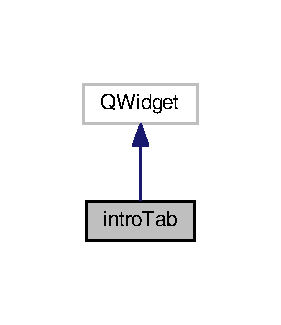
\includegraphics[width=135pt]{classintroTab__inherit__graph}
\end{center}
\end{figure}


Collaboration diagram for intro\+Tab\+:\nopagebreak
\begin{figure}[H]
\begin{center}
\leavevmode
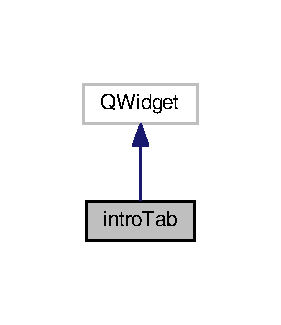
\includegraphics[width=135pt]{classintroTab__coll__graph}
\end{center}
\end{figure}
\subsection*{Signals}
\begin{DoxyCompactItemize}
\item 
\mbox{\Hypertarget{classintroTab_a76fc0e265d1a76c808dae9671b9248b4}\label{classintroTab_a76fc0e265d1a76c808dae9671b9248b4}} 
void {\bfseries set\+Tab} (int)
\end{DoxyCompactItemize}
\subsection*{Public Member Functions}
\begin{DoxyCompactItemize}
\item 
\mbox{\Hypertarget{classintroTab_aab649dfc9a71489cd08871faca7684a9}\label{classintroTab_aab649dfc9a71489cd08871faca7684a9}} 
{\bfseries intro\+Tab} (Q\+Widget $\ast$parent=0)
\item 
\mbox{\Hypertarget{classintroTab_a3ff2701ec758f8a9e2e663b9dac7e84c}\label{classintroTab_a3ff2701ec758f8a9e2e663b9dac7e84c}} 
void {\bfseries change\+Tab} (int tab)
\end{DoxyCompactItemize}
\subsection*{Public Attributes}
\begin{DoxyCompactItemize}
\item 
\mbox{\Hypertarget{classintroTab_a62af4606a05e32cec1902e4b3a9c7a7c}\label{classintroTab_a62af4606a05e32cec1902e4b3a9c7a7c}} 
Q\+Label $\ast$ {\bfseries label}
\item 
\mbox{\Hypertarget{classintroTab_afac3999d62248dee277ea3ad4a37ed60}\label{classintroTab_afac3999d62248dee277ea3ad4a37ed60}} 
Q\+Label $\ast$ {\bfseries image\+\_\+label}
\item 
\mbox{\Hypertarget{classintroTab_aec6d0b3cd99b3d517cb4ca29e445b990}\label{classintroTab_aec6d0b3cd99b3d517cb4ca29e445b990}} 
Q\+Label $\ast$ {\bfseries description\+\_\+label}
\item 
\mbox{\Hypertarget{classintroTab_a1209ccb530831d7c642817f47ecada86}\label{classintroTab_a1209ccb530831d7c642817f47ecada86}} 
Q\+V\+Box\+Layout $\ast$ {\bfseries main\+Layout}
\item 
\mbox{\Hypertarget{classintroTab_a7ddb2126611ddecd31543dc6210c0c7e}\label{classintroTab_a7ddb2126611ddecd31543dc6210c0c7e}} 
Q\+Main\+Window $\ast$ {\bfseries main\+Window}
\end{DoxyCompactItemize}


The documentation for this class was generated from the following files\+:\begin{DoxyCompactItemize}
\item 
introtab.\+h\item 
introtab.\+cpp\item 
moc\+\_\+introtab.\+cpp\end{DoxyCompactItemize}

\hypertarget{classLinuxConf}{}\section{Linux\+Conf Class Reference}
\label{classLinuxConf}\index{Linux\+Conf@{Linux\+Conf}}


Collaboration diagram for Linux\+Conf\+:\nopagebreak
\begin{figure}[H]
\begin{center}
\leavevmode
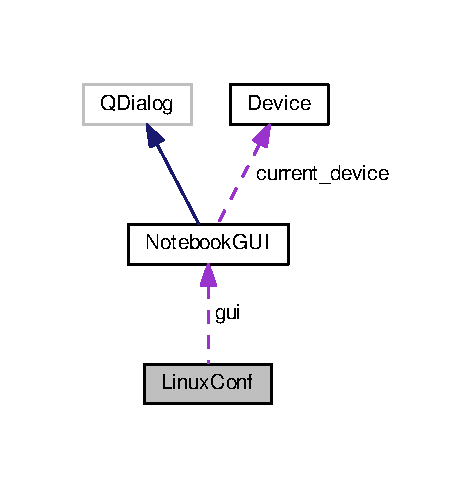
\includegraphics[width=227pt]{classLinuxConf__coll__graph}
\end{center}
\end{figure}
\subsection*{Static Public Member Functions}
\begin{DoxyCompactItemize}
\item 
\mbox{\Hypertarget{classLinuxConf_a6c618d4ab944d98f18830e33c1102609}\label{classLinuxConf_a6c618d4ab944d98f18830e33c1102609}} 
static void {\bfseries on\+\_\+button\+\_\+clicked} (std\+::string command, \hyperlink{classDevice}{Device} \&device)
\end{DoxyCompactItemize}
\subsection*{Public Attributes}
\begin{DoxyCompactItemize}
\item 
\mbox{\Hypertarget{classLinuxConf_a59770ab7bb16baf7f3ceb6cb757216e6}\label{classLinuxConf_a59770ab7bb16baf7f3ceb6cb757216e6}} 
\hyperlink{classNotebookGUI}{Notebook\+G\+UI} {\bfseries gui}
\end{DoxyCompactItemize}


The documentation for this class was generated from the following files\+:\begin{DoxyCompactItemize}
\item 
Linuxconf.\+h\item 
Linuxconf.\+cpp\end{DoxyCompactItemize}

\hypertarget{structMyException}{}\section{My\+Exception Struct Reference}
\label{structMyException}\index{My\+Exception@{My\+Exception}}


exception handling class.  




Inheritance diagram for My\+Exception\+:\nopagebreak
\begin{figure}[H]
\begin{center}
\leavevmode
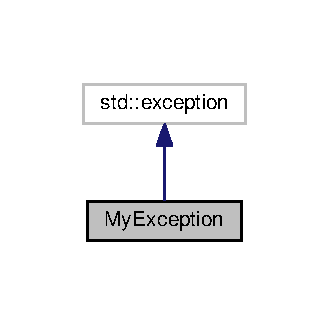
\includegraphics[width=158pt]{structMyException__inherit__graph}
\end{center}
\end{figure}


Collaboration diagram for My\+Exception\+:\nopagebreak
\begin{figure}[H]
\begin{center}
\leavevmode
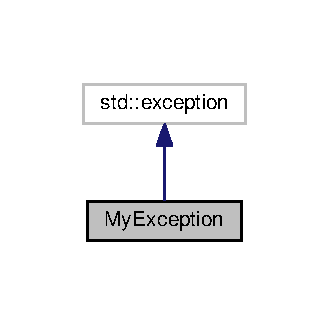
\includegraphics[width=158pt]{structMyException__coll__graph}
\end{center}
\end{figure}
\subsection*{Public Member Functions}
\begin{DoxyCompactItemize}
\item 
\mbox{\Hypertarget{structMyException_ad71a4be73b05417e6ac5ebdd44bb02ac}\label{structMyException_ad71a4be73b05417e6ac5ebdd44bb02ac}} 
{\bfseries My\+Exception} (std\+::string ss)
\item 
\mbox{\Hypertarget{structMyException_ae4760fb255c8fafae1e8307642172d90}\label{structMyException_ae4760fb255c8fafae1e8307642172d90}} 
const char $\ast$ {\bfseries what} () const  throw ()
\end{DoxyCompactItemize}
\subsection*{Public Attributes}
\begin{DoxyCompactItemize}
\item 
\mbox{\Hypertarget{structMyException_a99afdf5c0f4a14da793d7487ce398e3e}\label{structMyException_a99afdf5c0f4a14da793d7487ce398e3e}} 
std\+::string {\bfseries s}
\end{DoxyCompactItemize}


\subsection{Detailed Description}
exception handling class. 

The documentation for this struct was generated from the following file\+:\begin{DoxyCompactItemize}
\item 
device.\+cpp\end{DoxyCompactItemize}

\hypertarget{classNotebookGUI}{}\section{Notebook\+G\+UI Class Reference}
\label{classNotebookGUI}\index{Notebook\+G\+UI@{Notebook\+G\+UI}}


Inheritance diagram for Notebook\+G\+UI\+:\nopagebreak
\begin{figure}[H]
\begin{center}
\leavevmode
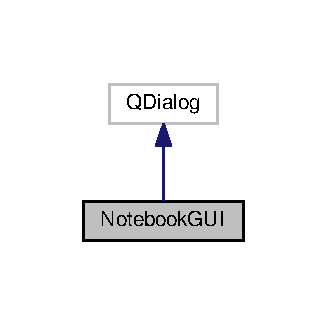
\includegraphics[width=157pt]{classNotebookGUI__inherit__graph}
\end{center}
\end{figure}


Collaboration diagram for Notebook\+G\+UI\+:\nopagebreak
\begin{figure}[H]
\begin{center}
\leavevmode
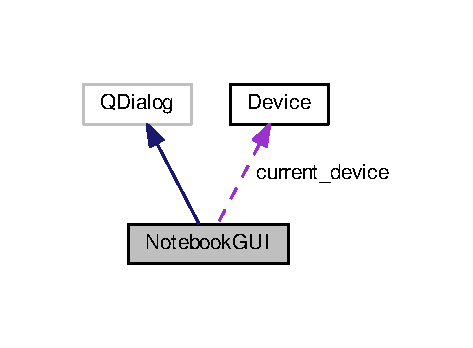
\includegraphics[width=227pt]{classNotebookGUI__coll__graph}
\end{center}
\end{figure}
\subsection*{Public Slots}
\begin{DoxyCompactItemize}
\item 
\mbox{\Hypertarget{classNotebookGUI_a884a0fcff797d5e04c649417b813bde6}\label{classNotebookGUI_a884a0fcff797d5e04c649417b813bde6}} 
void {\bfseries change\+Tab} (int index)
\item 
\mbox{\Hypertarget{classNotebookGUI_a7ff25fc8ea4287bd42d2e4deae59a65a}\label{classNotebookGUI_a7ff25fc8ea4287bd42d2e4deae59a65a}} 
void {\bfseries run\+Command} (\hyperlink{classDevice}{Device} device, string method, vector$<$ string $>$ parameters)
\item 
\mbox{\Hypertarget{classNotebookGUI_a3d367714a753d3bd1d6cdbc1a04a260a}\label{classNotebookGUI_a3d367714a753d3bd1d6cdbc1a04a260a}} 
void {\bfseries update\+Contributor} ()
\end{DoxyCompactItemize}
\subsection*{Signals}
\begin{DoxyCompactItemize}
\item 
\mbox{\Hypertarget{classNotebookGUI_abef5dbd76aefa47c910aeead0ad93023}\label{classNotebookGUI_abef5dbd76aefa47c910aeead0ad93023}} 
void {\bfseries updated\+Contributor} (\hyperlink{classDevice}{Device} device)
\item 
\mbox{\Hypertarget{classNotebookGUI_af35799599bf211bb41938c1bd3c5b3c3}\label{classNotebookGUI_af35799599bf211bb41938c1bd3c5b3c3}} 
void {\bfseries show\+Buttons} (vector$<$ string $>$, bool)
\item 
\mbox{\Hypertarget{classNotebookGUI_a03364e41a531b82671c130adb63f8fc7}\label{classNotebookGUI_a03364e41a531b82671c130adb63f8fc7}} 
void {\bfseries update\+Device} (\hyperlink{classDevice}{Device})
\item 
\mbox{\Hypertarget{classNotebookGUI_a4c798f9054beb2954af7d64eda562504}\label{classNotebookGUI_a4c798f9054beb2954af7d64eda562504}} 
void {\bfseries send\+To\+Console} (\hyperlink{classDevice}{Device}, string, vector$<$ string $>$)
\end{DoxyCompactItemize}
\subsection*{Public Member Functions}
\begin{DoxyCompactItemize}
\item 
\mbox{\Hypertarget{classNotebookGUI_a87df8290721912a46164f7c34ad4df42}\label{classNotebookGUI_a87df8290721912a46164f7c34ad4df42}} 
void {\bfseries set\+Device} (\hyperlink{classDevice}{Device} device, string $\ast$test\+\_\+parameters)
\item 
\mbox{\Hypertarget{classNotebookGUI_a53202e15038548e1bc83bad3cfb6397b}\label{classNotebookGUI_a53202e15038548e1bc83bad3cfb6397b}} 
{\bfseries Notebook\+G\+UI} (const Q\+String name)
\item 
\mbox{\Hypertarget{classNotebookGUI_a44dc0f2eb98b47a447c2088216512f2e}\label{classNotebookGUI_a44dc0f2eb98b47a447c2088216512f2e}} 
void {\bfseries show\+Result\+Buttons} ()
\item 
\mbox{\Hypertarget{classNotebookGUI_a189f72dabffb1e71e02a1705288f021f}\label{classNotebookGUI_a189f72dabffb1e71e02a1705288f021f}} 
void {\bfseries show\+Fail\+Button} ()
\end{DoxyCompactItemize}
\subsection*{Public Attributes}
\begin{DoxyCompactItemize}
\item 
\mbox{\Hypertarget{classNotebookGUI_a21113dc7b67c66e88563059644af1f26}\label{classNotebookGUI_a21113dc7b67c66e88563059644af1f26}} 
Q\+Tab\+Widget $\ast$ {\bfseries tab\+Widget}
\end{DoxyCompactItemize}
\subsection*{Protected Attributes}
\begin{DoxyCompactItemize}
\item 
\mbox{\Hypertarget{classNotebookGUI_a2beef42206665f7937636774a3881e5b}\label{classNotebookGUI_a2beef42206665f7937636774a3881e5b}} 
\hyperlink{classDevice}{Device} {\bfseries current\+\_\+device}
\item 
\mbox{\Hypertarget{classNotebookGUI_a49bf58ca1ac34fb077e82e7fd864eea4}\label{classNotebookGUI_a49bf58ca1ac34fb077e82e7fd864eea4}} 
string {\bfseries install\+\_\+method}
\item 
\mbox{\Hypertarget{classNotebookGUI_a3a8ce87e5a4a03d8d500268bcfa835b3}\label{classNotebookGUI_a3a8ce87e5a4a03d8d500268bcfa835b3}} 
vector$<$ string $>$ {\bfseries install\+\_\+details}
\end{DoxyCompactItemize}


The documentation for this class was generated from the following files\+:\begin{DoxyCompactItemize}
\item 
Notebook\+G\+U\+I.\+h\item 
moc\+\_\+\+Notebook\+G\+U\+I.\+cpp\item 
Notebook\+G\+U\+I.\+cpp\end{DoxyCompactItemize}

\hypertarget{structqt__meta__stringdata__ConsoleTab__t}{}\section{qt\+\_\+meta\+\_\+stringdata\+\_\+\+Console\+Tab\+\_\+t Struct Reference}
\label{structqt__meta__stringdata__ConsoleTab__t}\index{qt\+\_\+meta\+\_\+stringdata\+\_\+\+Console\+Tab\+\_\+t@{qt\+\_\+meta\+\_\+stringdata\+\_\+\+Console\+Tab\+\_\+t}}
\subsection*{Public Attributes}
\begin{DoxyCompactItemize}
\item 
\mbox{\Hypertarget{structqt__meta__stringdata__ConsoleTab__t_ad8ce80446f0554c014d086e889a3c41b}\label{structqt__meta__stringdata__ConsoleTab__t_ad8ce80446f0554c014d086e889a3c41b}} 
Q\+Byte\+Array\+Data {\bfseries data} \mbox{[}16\mbox{]}
\item 
\mbox{\Hypertarget{structqt__meta__stringdata__ConsoleTab__t_aee5160931d50cc0882dfa17fa9051b12}\label{structqt__meta__stringdata__ConsoleTab__t_aee5160931d50cc0882dfa17fa9051b12}} 
char {\bfseries stringdata0} \mbox{[}154\mbox{]}
\end{DoxyCompactItemize}


The documentation for this struct was generated from the following file\+:\begin{DoxyCompactItemize}
\item 
moc\+\_\+\+Console\+Tab.\+cpp\end{DoxyCompactItemize}

\hypertarget{structqt__meta__stringdata__ContributorTab2__t}{}\section{qt\+\_\+meta\+\_\+stringdata\+\_\+\+Contributor\+Tab2\+\_\+t Struct Reference}
\label{structqt__meta__stringdata__ContributorTab2__t}\index{qt\+\_\+meta\+\_\+stringdata\+\_\+\+Contributor\+Tab2\+\_\+t@{qt\+\_\+meta\+\_\+stringdata\+\_\+\+Contributor\+Tab2\+\_\+t}}
\subsection*{Public Attributes}
\begin{DoxyCompactItemize}
\item 
\mbox{\Hypertarget{structqt__meta__stringdata__ContributorTab2__t_a54ecc9bf723828e3ada381171e472fd9}\label{structqt__meta__stringdata__ContributorTab2__t_a54ecc9bf723828e3ada381171e472fd9}} 
Q\+Byte\+Array\+Data {\bfseries data} \mbox{[}9\mbox{]}
\item 
\mbox{\Hypertarget{structqt__meta__stringdata__ContributorTab2__t_aec0150009a5a461e070dbd8e4dc7e822}\label{structqt__meta__stringdata__ContributorTab2__t_aec0150009a5a461e070dbd8e4dc7e822}} 
char {\bfseries stringdata0} \mbox{[}106\mbox{]}
\end{DoxyCompactItemize}


The documentation for this struct was generated from the following file\+:\begin{DoxyCompactItemize}
\item 
moc\+\_\+\+Contributor\+Tab2.\+cpp\end{DoxyCompactItemize}

\hypertarget{structqt__meta__stringdata__introTab__t}{}\section{qt\+\_\+meta\+\_\+stringdata\+\_\+intro\+Tab\+\_\+t Struct Reference}
\label{structqt__meta__stringdata__introTab__t}\index{qt\+\_\+meta\+\_\+stringdata\+\_\+intro\+Tab\+\_\+t@{qt\+\_\+meta\+\_\+stringdata\+\_\+intro\+Tab\+\_\+t}}
\subsection*{Public Attributes}
\begin{DoxyCompactItemize}
\item 
\mbox{\Hypertarget{structqt__meta__stringdata__introTab__t_adb86563bfaf47b86d105822d1da75661}\label{structqt__meta__stringdata__introTab__t_adb86563bfaf47b86d105822d1da75661}} 
Q\+Byte\+Array\+Data {\bfseries data} \mbox{[}3\mbox{]}
\item 
\mbox{\Hypertarget{structqt__meta__stringdata__introTab__t_af683b0579164a88d1289719f7a73e4f6}\label{structqt__meta__stringdata__introTab__t_af683b0579164a88d1289719f7a73e4f6}} 
char {\bfseries stringdata0} \mbox{[}17\mbox{]}
\end{DoxyCompactItemize}


The documentation for this struct was generated from the following file\+:\begin{DoxyCompactItemize}
\item 
moc\+\_\+introtab.\+cpp\end{DoxyCompactItemize}

\hypertarget{structqt__meta__stringdata__NotebookGUI__t}{}\section{qt\+\_\+meta\+\_\+stringdata\+\_\+\+Notebook\+G\+U\+I\+\_\+t Struct Reference}
\label{structqt__meta__stringdata__NotebookGUI__t}\index{qt\+\_\+meta\+\_\+stringdata\+\_\+\+Notebook\+G\+U\+I\+\_\+t@{qt\+\_\+meta\+\_\+stringdata\+\_\+\+Notebook\+G\+U\+I\+\_\+t}}
\subsection*{Public Attributes}
\begin{DoxyCompactItemize}
\item 
\mbox{\Hypertarget{structqt__meta__stringdata__NotebookGUI__t_ac1e5bd12bc64dcc34c29c0d466905d4f}\label{structqt__meta__stringdata__NotebookGUI__t_ac1e5bd12bc64dcc34c29c0d466905d4f}} 
Q\+Byte\+Array\+Data {\bfseries data} \mbox{[}16\mbox{]}
\item 
\mbox{\Hypertarget{structqt__meta__stringdata__NotebookGUI__t_abea86eea86dfb716c21340a08e8c7dfc}\label{structqt__meta__stringdata__NotebookGUI__t_abea86eea86dfb716c21340a08e8c7dfc}} 
char {\bfseries stringdata0} \mbox{[}170\mbox{]}
\end{DoxyCompactItemize}


The documentation for this struct was generated from the following file\+:\begin{DoxyCompactItemize}
\item 
moc\+\_\+\+Notebook\+G\+U\+I.\+cpp\end{DoxyCompactItemize}

\hypertarget{structqt__meta__stringdata__RestoreTab__t}{}\section{qt\+\_\+meta\+\_\+stringdata\+\_\+\+Restore\+Tab\+\_\+t Struct Reference}
\label{structqt__meta__stringdata__RestoreTab__t}\index{qt\+\_\+meta\+\_\+stringdata\+\_\+\+Restore\+Tab\+\_\+t@{qt\+\_\+meta\+\_\+stringdata\+\_\+\+Restore\+Tab\+\_\+t}}
\subsection*{Public Attributes}
\begin{DoxyCompactItemize}
\item 
\mbox{\Hypertarget{structqt__meta__stringdata__RestoreTab__t_ae65b519ce9ee3f62ede6129255212be8}\label{structqt__meta__stringdata__RestoreTab__t_ae65b519ce9ee3f62ede6129255212be8}} 
Q\+Byte\+Array\+Data {\bfseries data} \mbox{[}10\mbox{]}
\item 
\mbox{\Hypertarget{structqt__meta__stringdata__RestoreTab__t_a1b27dc533cd8198d21f7dd99ad1c4b53}\label{structqt__meta__stringdata__RestoreTab__t_a1b27dc533cd8198d21f7dd99ad1c4b53}} 
char {\bfseries stringdata0} \mbox{[}88\mbox{]}
\end{DoxyCompactItemize}


The documentation for this struct was generated from the following file\+:\begin{DoxyCompactItemize}
\item 
moc\+\_\+\+Restore\+Tab.\+cpp\end{DoxyCompactItemize}

\hypertarget{structqt__meta__stringdata__RunTab__t}{}\section{qt\+\_\+meta\+\_\+stringdata\+\_\+\+Run\+Tab\+\_\+t Struct Reference}
\label{structqt__meta__stringdata__RunTab__t}\index{qt\+\_\+meta\+\_\+stringdata\+\_\+\+Run\+Tab\+\_\+t@{qt\+\_\+meta\+\_\+stringdata\+\_\+\+Run\+Tab\+\_\+t}}
\subsection*{Public Attributes}
\begin{DoxyCompactItemize}
\item 
\mbox{\Hypertarget{structqt__meta__stringdata__RunTab__t_a6f6c97baa156b1e17e04ddac9f025e70}\label{structqt__meta__stringdata__RunTab__t_a6f6c97baa156b1e17e04ddac9f025e70}} 
Q\+Byte\+Array\+Data {\bfseries data} \mbox{[}10\mbox{]}
\item 
\mbox{\Hypertarget{structqt__meta__stringdata__RunTab__t_a6138f3ebee1549de7407a802ff857809}\label{structqt__meta__stringdata__RunTab__t_a6138f3ebee1549de7407a802ff857809}} 
char {\bfseries stringdata0} \mbox{[}94\mbox{]}
\end{DoxyCompactItemize}


The documentation for this struct was generated from the following file\+:\begin{DoxyCompactItemize}
\item 
moc\+\_\+\+Run\+Config\+Tab.\+cpp\end{DoxyCompactItemize}

\hypertarget{classQuestionBox}{}\section{Question\+Box Class Reference}
\label{classQuestionBox}\index{Question\+Box@{Question\+Box}}


Inheritance diagram for Question\+Box\+:\nopagebreak
\begin{figure}[H]
\begin{center}
\leavevmode
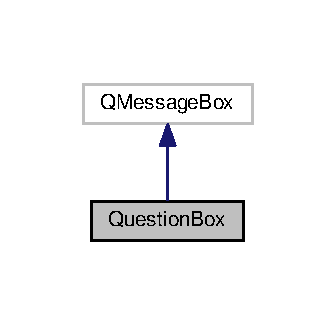
\includegraphics[width=161pt]{classQuestionBox__inherit__graph}
\end{center}
\end{figure}


Collaboration diagram for Question\+Box\+:\nopagebreak
\begin{figure}[H]
\begin{center}
\leavevmode
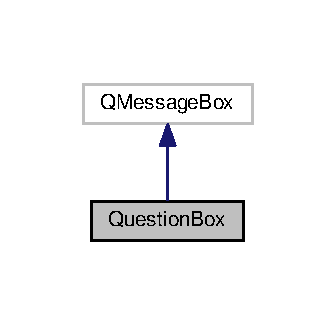
\includegraphics[width=161pt]{classQuestionBox__coll__graph}
\end{center}
\end{figure}
\subsection*{Public Member Functions}
\begin{DoxyCompactItemize}
\item 
\mbox{\Hypertarget{classQuestionBox_abe8853e77a48536473fdf35162b91bcd}\label{classQuestionBox_abe8853e77a48536473fdf35162b91bcd}} 
{\bfseries Question\+Box} (string message)
\end{DoxyCompactItemize}


The documentation for this class was generated from the following files\+:\begin{DoxyCompactItemize}
\item 
Question\+Box.\+h\item 
Question\+Box.\+cpp\end{DoxyCompactItemize}

\hypertarget{classRestoreGUI}{}\section{Restore\+G\+UI Class Reference}
\label{classRestoreGUI}\index{Restore\+G\+UI@{Restore\+G\+UI}}
\subsection*{Public Member Functions}
\begin{DoxyCompactItemize}
\item 
\mbox{\Hypertarget{classRestoreGUI_ab54fe7c54fd935a16087b8e3af3dfe64}\label{classRestoreGUI_ab54fe7c54fd935a16087b8e3af3dfe64}} 
{\bfseries Restore\+G\+UI} (std\+::map$<$ std\+::string, \hyperlink{classDevice}{Device} $>$ hashmap)
\end{DoxyCompactItemize}
\subsection*{Static Public Member Functions}
\begin{DoxyCompactItemize}
\item 
\mbox{\Hypertarget{classRestoreGUI_ac6b5762f54f83312872ca663890b8d66}\label{classRestoreGUI_ac6b5762f54f83312872ca663890b8d66}} 
static bool {\bfseries Command\+Line\+Install} (std\+::map$<$ string, \hyperlink{classDevice}{Device} $>$ device\+\_\+map)
\item 
\mbox{\Hypertarget{classRestoreGUI_a7cf25f915cd38767c2615bd385822fa4}\label{classRestoreGUI_a7cf25f915cd38767c2615bd385822fa4}} 
static string {\bfseries Do\+Restore} (string restorefile)
\end{DoxyCompactItemize}
\subsection*{Protected Member Functions}
\begin{DoxyCompactItemize}
\item 
\mbox{\Hypertarget{classRestoreGUI_a51dfeb36a85cee02b2a644385a42597f}\label{classRestoreGUI_a51dfeb36a85cee02b2a644385a42597f}} 
void {\bfseries on\+\_\+button\+\_\+clicked} (std\+::string command, \hyperlink{classDevice}{Device} device)
\end{DoxyCompactItemize}
\subsection*{Protected Attributes}
\begin{DoxyCompactItemize}
\item 
\mbox{\Hypertarget{classRestoreGUI_a051821a4af9951efe8afd792b6e5afe0}\label{classRestoreGUI_a051821a4af9951efe8afd792b6e5afe0}} 
std\+::set$<$ \hyperlink{classDevice}{Device} $>$ {\bfseries data}
\end{DoxyCompactItemize}


The documentation for this class was generated from the following files\+:\begin{DoxyCompactItemize}
\item 
Restore\+Cmd.\+h\item 
Restore\+Cmd.\+cpp\end{DoxyCompactItemize}

\hypertarget{classRestoreTab}{}\section{Restore\+Tab Class Reference}
\label{classRestoreTab}\index{Restore\+Tab@{Restore\+Tab}}


Inheritance diagram for Restore\+Tab\+:\nopagebreak
\begin{figure}[H]
\begin{center}
\leavevmode
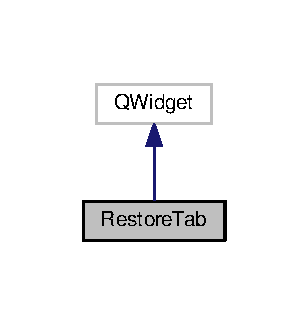
\includegraphics[width=148pt]{classRestoreTab__inherit__graph}
\end{center}
\end{figure}


Collaboration diagram for Restore\+Tab\+:\nopagebreak
\begin{figure}[H]
\begin{center}
\leavevmode
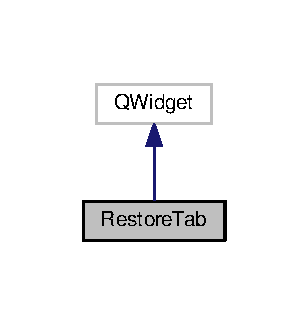
\includegraphics[width=148pt]{classRestoreTab__coll__graph}
\end{center}
\end{figure}
\subsection*{Public Slots}
\begin{DoxyCompactItemize}
\item 
\mbox{\Hypertarget{classRestoreTab_a549e7118c5e8a28af1479a976e396963}\label{classRestoreTab_a549e7118c5e8a28af1479a976e396963}} 
void {\bfseries update} (string message)
\end{DoxyCompactItemize}
\subsection*{Signals}
\begin{DoxyCompactItemize}
\item 
\mbox{\Hypertarget{classRestoreTab_ab4823d1d9bea7a4a5a831aa03a51861b}\label{classRestoreTab_ab4823d1d9bea7a4a5a831aa03a51861b}} 
void {\bfseries send\+Command} (\hyperlink{classDevice}{Device}, string, vector$<$ string $>$)
\item 
\mbox{\Hypertarget{classRestoreTab_a165346467b7ce01ec33fde98e234e4e5}\label{classRestoreTab_a165346467b7ce01ec33fde98e234e4e5}} 
void {\bfseries update\+Screen} (void)
\item 
\mbox{\Hypertarget{classRestoreTab_aaef0bb2a23fb3b2c4dc4decd8d4973c5}\label{classRestoreTab_aaef0bb2a23fb3b2c4dc4decd8d4973c5}} 
void {\bfseries set\+Tab} (int)
\end{DoxyCompactItemize}
\subsection*{Public Member Functions}
\begin{DoxyCompactItemize}
\item 
\mbox{\Hypertarget{classRestoreTab_acda42485891361316db7775e695c4530}\label{classRestoreTab_acda42485891361316db7775e695c4530}} 
{\bfseries Restore\+Tab} (Q\+Widget $\ast$parent=0)
\item 
\mbox{\Hypertarget{classRestoreTab_aa1bb831ba9b097a7d5f565ab452d34df}\label{classRestoreTab_aa1bb831ba9b097a7d5f565ab452d34df}} 
string {\bfseries Do\+Restore} (\hyperlink{classDevice}{Device} device)
\item 
\mbox{\Hypertarget{classRestoreTab_abc2f0056b937d2ea5c9550efc271d72e}\label{classRestoreTab_abc2f0056b937d2ea5c9550efc271d72e}} 
void {\bfseries Restore\+Button} (\hyperlink{classDevice}{Device} device)
\item 
\mbox{\Hypertarget{classRestoreTab_aed26e09af67d9cd7e11bd36ca6b4eecc}\label{classRestoreTab_aed26e09af67d9cd7e11bd36ca6b4eecc}} 
void {\bfseries Success\+Button} (\hyperlink{classDevice}{Device} device)
\item 
\mbox{\Hypertarget{classRestoreTab_a01c85e4378871f74a9fadf1ccf1dc3a9}\label{classRestoreTab_a01c85e4378871f74a9fadf1ccf1dc3a9}} 
void {\bfseries Fail\+Button} (\hyperlink{classDevice}{Device} device)
\item 
\mbox{\Hypertarget{classRestoreTab_af3b0de7700a051ffba65d2a987868858}\label{classRestoreTab_af3b0de7700a051ffba65d2a987868858}} 
void {\bfseries clear\+Layout} (Q\+Layout $\ast$layout, bool delete\+Widgets)
\end{DoxyCompactItemize}
\subsection*{Public Attributes}
\begin{DoxyCompactItemize}
\item 
\mbox{\Hypertarget{classRestoreTab_a66ca672d4dc55694dfdfdd7ea3181d04}\label{classRestoreTab_a66ca672d4dc55694dfdfdd7ea3181d04}} 
Q\+V\+Box\+Layout $\ast$ {\bfseries main\+Layout}
\end{DoxyCompactItemize}


The documentation for this class was generated from the following files\+:\begin{DoxyCompactItemize}
\item 
Restore\+Tab.\+h\item 
moc\+\_\+\+Restore\+Tab.\+cpp\item 
Restore\+Tab.\+cpp\end{DoxyCompactItemize}

\hypertarget{classRunConfig}{}\section{Run\+Config Class Reference}
\label{classRunConfig}\index{Run\+Config@{Run\+Config}}
\subsection*{Public Member Functions}
\begin{DoxyCompactItemize}
\item 
\mbox{\Hypertarget{classRunConfig_a482650ee4f8468857fb60fc6a5a8b62a}\label{classRunConfig_a482650ee4f8468857fb60fc6a5a8b62a}} 
std\+::string {\bfseries exec} (const char $\ast$cmd)
\end{DoxyCompactItemize}
\subsection*{Static Public Member Functions}
\begin{DoxyCompactItemize}
\item 
\mbox{\Hypertarget{classRunConfig_a5bf30574ec8400f70c03fa73aec39143}\label{classRunConfig_a5bf30574ec8400f70c03fa73aec39143}} 
static vector$<$ string $>$ {\bfseries install} (\hyperlink{classDevice}{Device} \&m\+\_\+device)
\item 
\mbox{\Hypertarget{classRunConfig_a4faba2a90a4a9f7f5848d98afe68bbe6}\label{classRunConfig_a4faba2a90a4a9f7f5848d98afe68bbe6}} 
static vector$<$ string $>$ {\bfseries uninstall} (\hyperlink{classDevice}{Device} \&m\+\_\+device)
\item 
\mbox{\Hypertarget{classRunConfig_a09e13b480e957af436d9fa072f3c803b}\label{classRunConfig_a09e13b480e957af436d9fa072f3c803b}} 
static vector$<$ string $>$ {\bfseries upgrade} (\hyperlink{classDevice}{Device} \&m\+\_\+device)
\item 
\mbox{\Hypertarget{classRunConfig_adc4527f1397bf44a015659fa67cfcfd8}\label{classRunConfig_adc4527f1397bf44a015659fa67cfcfd8}} 
static vector$<$ string $>$ {\bfseries restore} (\hyperlink{classDevice}{Device} \&m\+\_\+device)
\item 
\mbox{\Hypertarget{classRunConfig_a630df6ad6f2bab17feba3c31c0a1fdf5}\label{classRunConfig_a630df6ad6f2bab17feba3c31c0a1fdf5}} 
static bool {\bfseries restore\+Cmd} (\hyperlink{classDevice}{Device} \&m\+\_\+device)
\end{DoxyCompactItemize}


The documentation for this class was generated from the following files\+:\begin{DoxyCompactItemize}
\item 
Run\+Config.\+h\item 
Run\+Config.\+cpp\end{DoxyCompactItemize}

\hypertarget{classRunTab}{}\section{Run\+Tab Class Reference}
\label{classRunTab}\index{Run\+Tab@{Run\+Tab}}


Inheritance diagram for Run\+Tab\+:\nopagebreak
\begin{figure}[H]
\begin{center}
\leavevmode
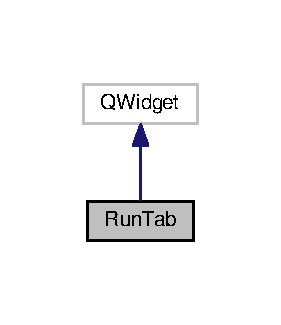
\includegraphics[width=135pt]{classRunTab__inherit__graph}
\end{center}
\end{figure}


Collaboration diagram for Run\+Tab\+:\nopagebreak
\begin{figure}[H]
\begin{center}
\leavevmode
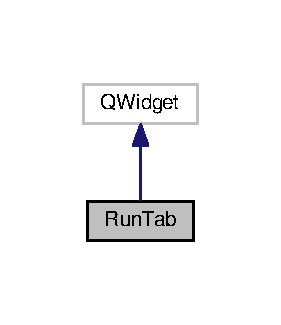
\includegraphics[width=135pt]{classRunTab__coll__graph}
\end{center}
\end{figure}
\subsection*{Public Slots}
\begin{DoxyCompactItemize}
\item 
\mbox{\Hypertarget{classRunTab_a365c10b3ea780707cfe7a78914570698}\label{classRunTab_a365c10b3ea780707cfe7a78914570698}} 
void {\bfseries install\+Button} (\hyperlink{classDevice}{Device})
\item 
\mbox{\Hypertarget{classRunTab_ad7c9fdbc6697b8ba55059c9c32abef3e}\label{classRunTab_ad7c9fdbc6697b8ba55059c9c32abef3e}} 
void {\bfseries uninstall\+Button} (\hyperlink{classDevice}{Device})
\item 
\mbox{\Hypertarget{classRunTab_a7f6949dfb2b64fd5b39844a7487257bf}\label{classRunTab_a7f6949dfb2b64fd5b39844a7487257bf}} 
void {\bfseries upgrade} (\hyperlink{classDevice}{Device})
\end{DoxyCompactItemize}
\subsection*{Signals}
\begin{DoxyCompactItemize}
\item 
\mbox{\Hypertarget{classRunTab_abb7ced8a7c06fbeb1efcbfd5a447f71e}\label{classRunTab_abb7ced8a7c06fbeb1efcbfd5a447f71e}} 
void {\bfseries set\+Tab} (int)
\item 
\mbox{\Hypertarget{classRunTab_a61b6e1f9775bf6d713fa0c5584078e1b}\label{classRunTab_a61b6e1f9775bf6d713fa0c5584078e1b}} 
void {\bfseries send\+Command} (\hyperlink{classDevice}{Device}, string, vector$<$ string $>$)
\end{DoxyCompactItemize}
\subsection*{Public Member Functions}
\begin{DoxyCompactItemize}
\item 
\mbox{\Hypertarget{classRunTab_a1114bef665434313ecdb37698f14b5d8}\label{classRunTab_a1114bef665434313ecdb37698f14b5d8}} 
{\bfseries Run\+Tab} (Q\+Widget $\ast$parent=0)
\item 
\mbox{\Hypertarget{classRunTab_a9543f31e26a44eb097b15a319a6d605e}\label{classRunTab_a9543f31e26a44eb097b15a319a6d605e}} 
void {\bfseries update\+Layout} ()
\item 
\mbox{\Hypertarget{classRunTab_a965700df008f390b46f64d097f58a9fe}\label{classRunTab_a965700df008f390b46f64d097f58a9fe}} 
void {\bfseries clear\+Layout} (Q\+Layout $\ast$layout, bool delete\+Widgets=true)
\end{DoxyCompactItemize}
\subsection*{Public Attributes}
\begin{DoxyCompactItemize}
\item 
\mbox{\Hypertarget{classRunTab_af04b75f887960ee096a63a8d900ccbab}\label{classRunTab_af04b75f887960ee096a63a8d900ccbab}} 
Q\+Widget $\ast$ {\bfseries m\+\_\+parent}
\item 
\mbox{\Hypertarget{classRunTab_ae0fa0fc309e5fd2e7b6ef0f64058eba3}\label{classRunTab_ae0fa0fc309e5fd2e7b6ef0f64058eba3}} 
Q\+Tab\+Widget $\ast$ {\bfseries tab\+Widget}
\item 
\mbox{\Hypertarget{classRunTab_a739838ef40e4196ba75464759dbb8004}\label{classRunTab_a739838ef40e4196ba75464759dbb8004}} 
Q\+Term\+Widget $\ast$ {\bfseries term\+Widget}
\item 
\mbox{\Hypertarget{classRunTab_a99ef949d7449cc935dab1540b520328e}\label{classRunTab_a99ef949d7449cc935dab1540b520328e}} 
Q\+V\+Box\+Layout $\ast$ {\bfseries main\+Layout}
\end{DoxyCompactItemize}


The documentation for this class was generated from the following files\+:\begin{DoxyCompactItemize}
\item 
Run\+Config\+Tab.\+h\item 
moc\+\_\+\+Run\+Config\+Tab.\+cpp\item 
Run\+Config\+Tab.\+cpp\end{DoxyCompactItemize}

%--- End generated contents ---

% Index
\backmatter
\newpage
\phantomsection
\clearemptydoublepage
\addcontentsline{toc}{chapter}{Index}
\printindex

\end{document}
